\documentclass{note}
\usepackage{mathptm,mydef,myenv}
%\usepackage{MinionPro}
\usepackage{color}
%\usepackage[scaled]{beramono}
%\usepackage[scaled]{ulgothic}
%\usepackage[ocr-a]{ocr}
%\usepackage{ocr}
%\usepackage{courier}
\usepackage{alltt}
\usepackage[all,knot]{xy}
\usepackage[T1]{fontenc}
\usepackage{graphicx}
\DeclareGraphicsExtensions{.png}

\usepackage{hyperref}
\hypersetup{
    colorlinks,
    citecolor=black,
    filecolor=black, 
    linkcolor=blue,
    urlcolor=black
}

%\setlength\oddsidemargin{-1.5cm}
%\setlength\evensidemargin{-1.5cm}
%\setlength\textwidth{19.3cm}
%\addtolength\topmargin{-1cm}
%\addtolength\textheight{2cm}
%\addtolength\columnsep{0.2cm}
%\newtheorem{theorem}{Theorem}
%\theoremstyle{definition}
%\newtheorem{definition}[theorem]{Definition}
%\def\EE{\mbox{\eufm{}E}}1

\begin{document}
\small


\title{\large\bf{}\textcolor{blue2}{Modem Design: UVM-to-UVMA Migration}}
\author{Cheoljoo Jeong}
%% $$\xy
%% %\vtop{\vbox{
%% \xygraph{!{0;/r0.7pc/:} !{\vover}[u]
%%   !{\hcap[-2]} [d] !{\vover-} [ruu] !{\hcap[2]}}
%% %}\smallskip}
%% \endxy$$
%% }
\date{}
%\date{\normalsize\today}
\maketitle

\tableofcontents

\section{Overview}
\subsection{Modem block diagram}
\centerline{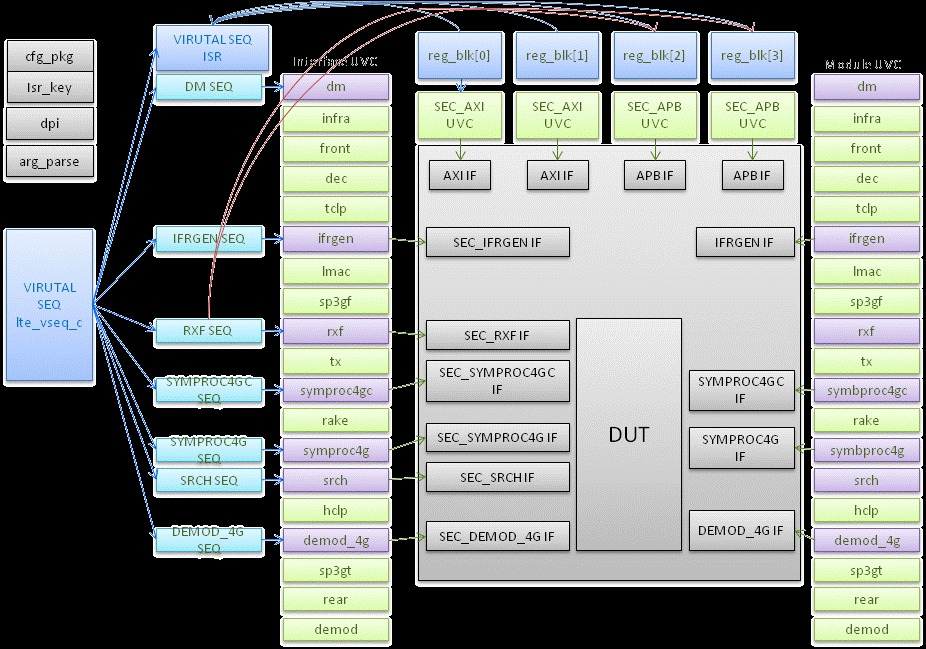
\includegraphics[width=12cm]{pics/modem}}
 
\subsection{Target files}
Files in \textcolor{red2}{red} are those in VCAD chamber.
\bit
\w \bb{Common interface}:
  \w \textcolor{red2}{\bb{sec\_modem/lib/common/common\_intf.sv}}
\w \bb{Interfaces}:
  \bit
  \w \textcolor{red2}{\bb{sec\_modem/lib/rxf/rxf\_intf.sv}}
  \w \bb{sec\_modem/lib/symbproc4g/symbproc4g\_intf.sv}
  \w \textcolor{red2}{\bb{sec\_modem/lib/symbproc4gc/symbproc4gc\_intf.sv}}
  \w \textcolor{red2}{\bb{sec\_modem/lib/demod\_4g/demod\_4g\_intf.sv}}
  \w \bb{sec\_modem/lib/ifrgen/ifrgen\_intf.sv}
  \w \bb{sec\_modem/lib/dm/dm\_intf.sv}
  \w \bb{uvc/sec\_dm/v201408/sv/sec\_dm\_intf.sv}
  \w \bb{uvc/sec\_demod/v201408/sv/sec\_demod\_intf.sv}
  \w \bb{uvc/sec\_rxf/v201408/sv/sec\_rxf\_intf.sv}
  \eit
\w \bb{Interface instantiations}:
  \bit
  \w \bb{sec\_modem/tb/top/intf\_inst.sv}
  \eit
\w \bb{Drivers}:
  \bit
  \w \textcolor{red2}{\bb{uvc/sec\_rxf/v201408/sv/sec\_rxf\_driver.sv}}
  \eit
\w \bb{Sequences}:
  \bit
  \w \bb{uvc/sec\_modem/lib/rxf/rxf\_\{seq,vseq\}\_lib.sv}
  \w \bb{uvc/sec\_modem/lib/symbproc4g/symbproc4g\_\{seq,vseq\}\_lib.sv}
  \w \bb{uvc/sec\_modem/lib/symbproc4gc/symbproc4gc\_\{seq,vseq\}\_lib.sv}
  \w
  \textcolor{red2}{\bb{uvc/sec\_modem/lib/demod\_4g/demod\_4g\_\{seq,vseq\}\_lib.sv}}
  (only seq\_lib given)
  \w \bb{uvc/sec\_modem/lib/dm/dm\_\{seq,vseq\}\_lib.sv}
  \w \bb{uvc/sec\_modem/lib/ifrgrn/ifrgen\_\{seq,vseq\}\_lib.sv}
  \eit
\eit


\section{Simulation Acceleration}
\subsection{Event wait with enable}
The following \verb+wait+ statement
\begin{verbatim}
  event ev;
  wait(ev.triggered);
\end{verbatim}
can be transformed
\begin{verbatim}
  @(ev);
\end{verbatim}


\section{UVM-to-UVMA Migration}

\subsection{Common Interface: common\_intf.sv}


\begin{alltt}
    // interrupt gen related
    bit vclk;
    always #2 vclk = ~vclk;
    `define INT_PULSE_GEN(NAME,SRC) \textbackslash
      bit r``NAME; \textbackslash
      always @ (posedge vclk) r``NAME <= SRC; \textbackslash
      wire NAME``Pulse = SRC&~r``NAME; 

    // this describes the checking point
    string check_point_name[MAX_CHECK_NUM];

    // the reference file name
    string check_ref_file_name[MAX_CHECK_NUM];

    // reference file type (0: 1 column, non zero: 2 columns)
    // 1: (i,q) pair
    // 2: (addr,data) pair
    int check_ref_file_type[MAX_CHECK_NUM];

    // reference file existence
    int check_ref_file_exists[MAX_CHECK_NUM];

    // reference data size (only for collect_type1)
    int check_ref_data_max_num[MAX_CHECK_NUM];
    initial foreach (check_ref_data_max_num[i]) check_ref_data_max_num[i] =
    -1;

    // key information to extract reference data from file
    string check_int_key_name[MAX_CHECK_NUM][$];
    int check_int_key_value[MAX_CHECK_NUM][$];
    string check_str_key_name[MAX_CHECK_NUM][$];
    string check_str_key_value[MAX_CHECK_NUM][$];

    // clock used for capturing the sample
    logic check_clk[MAX_CHECK_NUM];

    // the number of clocks we should skip after capturing the sample (usually
    0
)
    int check_clk_skip_num[MAX_CHECK_NUM];

    // signal indicating the start of the related logic (once or multiple
    times
throughout simulation)
    // if we use multiple generating start signal, we should use
    ``collect_type0''
 function at monitor.
    // else if we use one time generating start singal, we should use
    ``collect_t
ype1'' function at monitor.
    logic check_start[MAX_CHECK_NUM];

    // in-time data enable signal used for capturing the sample
    logic check_data_en[MAX_CHECK_NUM];

    // DUT signal to be captured
    logic [127:0] check_data[MAX_CHECK_NUM];
    logic [127:0] check_data_i[MAX_CHECK_NUM];
    logic [127:0] check_data_q[MAX_CHECK_NUM];

    // this is used for masking the invalid bit within 128-bit.
    logic [127:0] check_mask[MAX_CHECK_NUM];

    // symbol index within key group in testvector synchornizing with the
    curren
tly being captured DUT data
    int check_ref_data_idx[MAX_CHECK_NUM];
    // if some burst processing has its start-done pair, we should describe
    its
done signal.
    // this is only valid when multiple start signals exist
    (``collect_type0'')
    logic check_done[MAX_CHECK_NUM];

    // if some burst processing generates multiple done signals at a single
    star
t signal, we should define the number of done signal.
    // this is only valid when multiple start signals exist
    (``collect_type0'')
    int check_done_num[MAX_CHECK_NUM];

    // we should trigger this event, when we finish setting all parameters of
    ch
ecking point.
    // this starts monitor to capture the samples.
    event check_param_set_end[MAX_CHECK_NUM];

    // --------------------------------------------------
    // this parameters are for common
    // --------------------------------------------------
    bit checker_on;
    // this indicates whether this block is enabled.
    // we trigger on at body task of monitor.

    bit test_on;
    // this indicates whether reset is released.
    initial #5000ns test_on = checker_on;

\end{alltt}


\subsection{Interfaces}
\subsubsection{rxf\_intf.sv}
\begin{alltt}
interface rxf_intf(input logic nReset, input logic SystemClock, input clk,
input
 clkx2, input clkx4, input reset_n);

   // Common signals for Checkers
   parameter int MAX_CHECK_NUM = 32;
   parameter int MAX_CH_NUM = 6;

   `include ``common_intf.sv''

   logic   [119:0]       DUT_IntCpu;
   // yyn@DT logic   [108:0]       DUT_IntDsp;

   // internal node from SystemTime
   // yyn@DT logic oIntFreqShift;

   // modem primary IO interrupts
   `INT_PULSE_GEN (IntFreqShift,DUT_IntCpu[65])

   // ---------------------------------------
   // signals for driving L1
   // ---------------------------------------

   // Common
   // yyn@DT logic [31:0]            AntRxAdc[6];
   logic [MAX_CH_NUM-1:0]  Tclk;
   // yyn@DT logic [MAX_CH_NUM-1:0]  TtiTick;
   // yyn@DT logic                   GapEn   [MAX_CH_NUM];
   // yyn@DT logic                   AgapEn  [MAX_CH_NUM];
   // yyn@DT logic [2:0]             CurBW   [MAX_CH_NUM];
   // yyn@DT logic [2:0]             GapBW   [MAX_CH_NUM];
   // yyn@DT logic [2:0]             AgapBW  [MAX_CH_NUM];
   // yyn@DT logic [2:0]             PreBW   [MAX_CH_NUM];
   // yyn@DT logic [2:0]             InBW    [MAX_CH_NUM];
   // yyn@DT logic [MAX_CH_NUM-1:0]  InClk;
   // yyn@DT logic   [3:0]           PllSel  [MAX_CH_NUM];

   // yyn@DT logic   [2:0]           GapHold;
   logic                  GapRfStartTick, GapRfEndTick;
   // yyn@DT logic   [3:0]          GapInfo4G[3];
   logic   [3:0]          GapInfo[3];
   logic   [15:0]         ClkCount[3];

   // yyn@DT logic                  SyncIntCpu;
   // yyn@DT logic                  SyncIntDsp;

   // yyn@DT logic                   PnClkEn_3GF;
   logic                   PnClk2En_3GF;
   // yyn@DT logic                   PnClk4En_3GF;
   // For 3GF
   // Start signal from DUT
   logic                   _3gf_RxStart;
   logic                   _3gt_RxStart;
   // Start signal from DRV
   logic                   RX_START;
   // Monitoring signal
   // yyn@DT bit   [5:0]             DriveEn;
   // yyn@DT logic                   iRxfDCR0VClkEnable_0;
   // yyn@DT logic                   iRxfDCF0VClkEnable_0;
   bit [3:0] checker_3gf_start;
   bit checker_3gt_start;

   // RXF RxfStart signal modified to apply input with desired waveform

   // yyn@DT  logic w3GFRxStart;
   // yyn@DT  logic r3GFRxStartDly;
   // yyn@DT  logic r3GFRxStartDly2;
   // yyn@DT  always @(posedge clk) begin
   // yyn@DT    r3GFRxStartDly <= w3GFRxStart;
   // yyn@DT    r3GFRxStartDly2 <= r3GFRxStartDly;
   // yyn@DT  end
   // yyn@DT  logic w3GFRxStartEnlarged;
   // yyn@DT  assign w3GFRxStartEnlarged = w3GFRxStart | r3GFRxStartDly |
   r3GFRx
StartDly2;



   // 4G DVGA update
   bit                  RTG_CLK;
   logic   [3:0]        TTI_INDEX[3];
   logic   [2:0]        RxfTtiTick;
   logic   [2:0]        wTTI_TICK;
   logic   [2:0]        rTTI_TICK;
   logic   [2:0]        rTTI_INDEX_ON;

   always @(posedge RTG_CLK or negedge reset_n) begin
      if (!reset_n) begin
         rTTI_TICK <= 0;
         rTTI_INDEX_ON <= 0;
      end
      else begin
         rTTI_TICK <= wTTI_TICK;
         for (int i = 0; i < 3; i++)
            if (RxfTtiTick[i])
               rTTI_INDEX_ON[i] <= 1;
      end
   end


   // `INT_PULSE_GEN (IntBtfdEnd,DUT_IntCpu[34])
   // ---------------------------------------
   // + argument parsing
   // ---------------------------------------
   int front_rxf_uvc_cfg;
   int demod_rake_uvc_cfg;
   int demod_tclp_uvc_cfg;
   int check_3gf_rxf_start_offset[4] = '{12,12,12,12};
   int check_3gf_adcnum4fa[4];
   string rat_mode_cfg;
   string vec_dir;

   initial begin
      // check forcing argument
      if ($value$plusargs(``front_rxf_uvc_cfg=%d'', front_rxf_uvc_cfg));
      if ($value$plusargs(``demod_rake_uvc_cfg=%d'', demod_rake_uvc_cfg));
      if ($value$plusargs(``demod_tclp_uvc_cfg=%d'', demod_tclp_uvc_cfg));
      if ($value$plusargs(``check_3gf_rxf_start_offset0=%d'',
                                %check_3gf_rxf_start_
offset[0]));
      if ($value$plusargs(``check_3gf_rxf_start_offset1=%d'',
                                %check_3gf_rxf_start_
offset[1]));
      if ($value$plusargs(``check_3gf_rxf_start_offset2=%d'',
                                %check_3gf_rxf_start_
offset[2]));
      if ($value$plusargs(``check_3gf_rxf_start_offset3=%d'',
                                %check_3gf_rxf_start_
offset[3]));
      if ($value$plusargs(``check_3gf_adcnum4fa0=%d'',
                                %check_3gf_adcnum4fa[0]));
      if ($value$plusargs(``check_3gf_adcnum4fa1=%d'',
                                %check_3gf_adcnum4fa[1]));
      if ($value$plusargs(``check_3gf_adcnum4fa2=%d'',
                                %check_3gf_adcnum4fa[2]));
      if ($value$plusargs(``check_3gf_adcnum4fa3=%d'',
                                %check_3gf_adcnum4fa[3]));
      if ($value$plusargs(``rat_mode_cfg=%s'', rat_mode_cfg));
      if ($value$plusargs(``vec_dir=%s'', vec_dir));

      for (int i=0; i<4; i=i+1)
         $display(``rf_check_offset[%d] = %d'', i,
                                %check_3gf_rxf_start_offset[i]);

      if (front_rxf_uvc_cfg == 'd1 ||
          front_rxf_uvc_cfg == 'd3 ||
          front_rxf_uvc_cfg == 'd4)
          checker_on = 1;
   end
   initial begin
      #1;
      if (rat_mode_cfg==''3gf'') begin
        @ (posedge (demod_rake_uvc_cfg == 0 ? RX_START : _3gf_RxStart));
        fork
          begin @ (posedge Tclk[check_3gf_adcnum4fa[0]]); checker_3gf_start[0]
          =
 1; end
          begin @ (posedge Tclk[check_3gf_adcnum4fa[1]]); checker_3gf_start[1]
          =
 1; end
          begin @ (posedge Tclk[check_3gf_adcnum4fa[2]]); checker_3gf_start[2]
          =
 1; end
          begin @ (posedge Tclk[check_3gf_adcnum4fa[3]]); checker_3gf_start[3]
          =
 1; end
        join
      end
      if (rat_mode_cfg==''3gt'') begin
        @ (posedge (demod_tclp_uvc_cfg == 0 ? RX_START : _3gt_RxStart));
        @ (posedge Tclk[0]);
        checker_3gt_start = 1;
      end
   end

   // ------------------
   // checkers
   // ------------------
   // [0]: c0 a0
   // [1]: c0 a1
   // [2]: c1 a0
   // [3]: c1 a1
   // [4]: c2 a0
   // [5]: c2 a1
   // [6]: c3 a0
   // [7]: c3 a1
   logic [7:0] oFa0Rx0I;
   logic [7:0] oFa0Rx0Q;
   logic [7:0] oFa0Rx1I;
   logic [7:0] oFa0Rx1Q;
   logic [7:0] oFa1Rx0I;
   logic [7:0] oFa1Rx0Q;
   logic [7:0] oFa1Rx1I;
   logic [7:0] oFa1Rx1Q;
   logic [7:0] oFa2Rx0I;
   logic [7:0] oFa2Rx0Q;
   logic [7:0] oFa2Rx1I;
   logic [7:0] oFa2Rx1Q;
   logic [7:0] oFa3Rx0I;
   logic [7:0] oFa3Rx0Q;
   logic [7:0] oFa3Rx1I;
   logic [7:0] oFa3Rx1Q;
   `ifndef TEST_4G
   `ifdef _3G_OFFSET_FIND
      int check_3gf_rxf_free_cnt[4];
      bit [3:0] check_3gf_rxf_en;
      for (genvar i=0; i<4; i++)
         always @ (posedge PnClk2En_3GF iff checker_3gf_start[i]) begin
            check_3gf_rxf_free_cnt[i]++;
            if (check_3gf_rxf_free_cnt[i]>=check_3gf_rxf_start_offset[i])
               check_3gf_rxf_en[i] = 1;
         end

      int rxf_out_sample_num_3gf[3:0]; // for waveform check
      always @(negedge PnClk2En_3GF)
         for (int i=0; i<4; i++)
            rxf_out_sample_num_3gf[i] =
            check_3gf_rxf_free_cnt[i]-check_3gf_rxf_
start_offset[i]+1;

      int check_3gf_Fptr[8],check_3gf_line_valid[8];
      string
      check_3gf_line[8],check_3gf_vec_dir[8],check_3gf_str0[8],check_3gf_
str1[8];
      for (genvar i=0;i<8;i++) begin
         initial check_point_name[i] =
            $sformatf(``rx_filter output @ (carrier:%0d,
                                %antenna:%0d)'',i/2,i%2);
         assign check_clk[i] = PnClk2En_3GF;
         initial begin
            #1;
            check_ref_file_name[i] =
            $sformatf(``rxflt_dcr2_a0007_out3gf_a%0dc%0d
.txt'',i%2,i/2);
            void'($value$plusargs(``vec_dir=%s'', check_3gf_vec_dir[i]));
            check_ref_file_exists[i] = FILE_CHECK_LOCAL
            ($sformatf(``%0s/%0s'',che
ck_3gf_vec_dir[i],check_ref_file_name[i]));
            if (check_ref_file_exists[i]) begin
               check_3gf_Fptr[i] = $fopen
               ($sformatf(``%0s/%0s'',check_3gf_vec_dir
[i],check_ref_file_name[i]),''r'');
               check_ref_data_max_num[i] = 0;
               while ($fgets (check_3gf_line[i],check_3gf_Fptr[i])) begin
                  check_3gf_line_valid[i] = $sscanf (check_3gf_line[i],''%s
                                %%s'',c
heck_3gf_str0[i],check_3gf_str1[i]);
                  if (check_3gf_line_valid[i] == 2)
                     check_ref_data_max_num[i]++;
               end
               $fclose (check_3gf_Fptr[i]);
            end
            check_int_key_name[i].push_back(``fr'');
            check_int_key_value[i].push_back(0);
            check_ref_file_type[i] = 1;
         end
         assign check_start[i] = (demod_rake_uvc_cfg == 0 ? RX_START :
         _3gf_RxSt
art) & check_ref_file_exists[i];
         assign check_clk_skip_num[i] = 0;
         assign check_mask[i] = 8'hff;
         assign check_data_en[i] = check_3gf_rxf_en[i/2] &
         check_ref_file_exists
[i];
         always @ (posedge check_start[i] iff checker_on) begin
            check_ref_data_idx[i] = 0;
            ->check_param_set_end[i];
         end
         always @ (posedge check_clk[i] iff check_data_en[i] & checker_on)
            #1 check_ref_data_idx[i]++;
      end
      assign check_data_i[0] = oFa0Rx0I;
      assign check_data_q[0] = oFa0Rx0Q;
      assign check_data_i[1] = oFa0Rx1I;
      assign check_data_q[1] = oFa0Rx1Q;
      assign check_data_i[2] = oFa1Rx0I;
      assign check_data_q[2] = oFa1Rx0Q;
      assign check_data_i[3] = oFa1Rx1I;
      assign check_data_q[3] = oFa1Rx1Q;
      assign check_data_i[4] = oFa2Rx0I;
      assign check_data_q[4] = oFa2Rx0Q;
      assign check_data_i[5] = oFa2Rx1I;
      assign check_data_q[5] = oFa2Rx1Q;
      assign check_data_i[6] = oFa3Rx0I;
      assign check_data_q[6] = oFa3Rx0Q;
      assign check_data_i[7] = oFa3Rx1I;
      assign check_data_q[7] = oFa3Rx1Q;
   `endif // _3G_OFFSET_FIND
   `endif // TEST_4G

   // for 3gf rxf debugging
   `ifdef _3G_OFFSET_FIND
   // antenna0
   int Fptr0,line_valid0;
   string line0,str00,str01;
   int dvgaout3gf_array0_i[$];
   int dvgaout3gf_array0_q[$];
   logic [7:0] dvgaout3gf_a0c0_i;
   logic [7:0] dvgaout3gf_a0c0_q;
   int dvgaout3gf_cnt0;
   initial begin
      #1;
      Fptr0 = $fopen
      ($sformatf(``%0s/rxflt_dcr2_a0007_out3gf_a0c0.txt'',vec_dir),
``r'');
      if (Fptr0) begin
         while ($fgets(line0,Fptr0)) begin
            line_valid0 = $sscanf (line0,''%s %s'',str00,str01);
            if (line_valid0 == 2) begin
               dvgaout3gf_array0_i.push_back(str00.atohex());
               dvgaout3gf_array0_q.push_back(str01.atohex());
            end
         end
         $fclose(Fptr0);
      end
   end
   always @ (negedge PnClk2En_3GF iff checker_3gf_start&Fptr0) begin
      #4;
      dvgaout3gf_a0c0_i <=
      dvgaout3gf_array0_i[dvgaout3gf_cnt0-check_3gf_rxf_sta
rt_offset[0]+1];
      dvgaout3gf_a0c0_q <=
      dvgaout3gf_array0_q[dvgaout3gf_cnt0-check_3gf_rxf_sta
rt_offset[0]+1];
      dvgaout3gf_cnt0 <= dvgaout3gf_cnt0 + 1;
   end

   // antenna1
   int Fptr1,line_valid1;
   string line1,str10,str11;
   int dvgaout3gf_array1_i[$];
   int dvgaout3gf_array1_q[$];
   logic [7:0] dvgaout3gf_a1c0_i;
   logic [7:0] dvgaout3gf_a1c0_q;
   int dvgaout3gf_cnt1;
   initial begin
      #1;
      Fptr1 = $fopen
      ($sformatf(``%0s/rxflt_dcr2_a0007_out3gf_a1c0.txt'',vec_dir),
``r'');
      if (Fptr1) begin
         while ($fgets(line1,Fptr1)) begin
            line_valid1 = $sscanf (line1,''%s %s'',str10,str11);
            if (line_valid1 == 2) begin
               dvgaout3gf_array1_i.push_back(str10.atohex());
               dvgaout3gf_array1_q.push_back(str11.atohex());
            end
         end
         $fclose(Fptr1);
      end
   end
   always @ (negedge PnClk2En_3GF iff checker_3gf_start&Fptr1) begin
      #4;
      dvgaout3gf_a1c0_i <=
      dvgaout3gf_array1_i[dvgaout3gf_cnt1-check_3gf_rxf_sta
rt_offset[0]+1];
      dvgaout3gf_a1c0_q <=
      dvgaout3gf_array1_q[dvgaout3gf_cnt1-check_3gf_rxf_sta
rt_offset[0]+1];
      dvgaout3gf_cnt1 <= dvgaout3gf_cnt1 + 1;
   end
   `endif // _3G_OFFSET_FIND

   // For 3GT
   int ADC_index_3gt;

   `ifdef _3GT_CHAIN_
   logic [11:0] oRxIntOut0I;
   logic [11:0] oRxIntOut0Q;
   logic [11:0] oRxIntOut1I;
   logic [11:0] oRxIntOut1Q;

   logic        Chipx8Tick;

   localparam  intp_output_skip_length = 6;
   bit sar_adc_mode;
   int  intp_output_delay = 46;

   int check_3gt_rxf_free_cnt;
   bit check_3gt_rxf_en;
   int check_3gt_Fptr[2],check_3gt_line_valid[2];
   string check_3gt_line[2],check_3gt_vec_dir[2];
   logic [11:0] ref_RxIntOutI [0:1];
   logic [11:0] ref_RxIntOutQ [0:1];

    initial begin
      if ($value$plusargs(``sar_adc_mode=%0d'',sar_adc_mode));
      intp_output_delay = sar_adc_mode ? 49 : 46;
    end

   always @ (negedge Chipx8Tick iff checker_3gt_start) begin
      check_3gt_rxf_free_cnt++;
      //if (check_3gt_rxf_free_cnt>=check_3gt_rxf_start_offset) begin
      if (check_3gt_rxf_free_cnt>=intp_output_delay+intp_output_skip_length)
      beg
in
         check_3gt_rxf_en = 1;
      end
   end

   for (genvar i=0;i<2;i++) begin
      initial check_point_name[i+8] = $sformatf(``rx_filter output @
      (antenna:%0d
)'',i);
      assign check_clk[i+8] = Chipx8Tick;
      initial begin
         #1;
         check_ref_file_name[i+8] =
         $sformatf(``rxflt_intp_a0001_out_a%0dc0.txt'',
i);
         void'($value$plusargs(``vec_dir=%s'', check_3gt_vec_dir[i]));
         check_ref_file_exists[i+8] = FILE_CHECK_LOCAL
         ($sformatf(``%0s/%0s'',chec
k_3gt_vec_dir[i],check_ref_file_name[i+8]));
         if (check_ref_file_exists[i+8]) begin
            check_3gt_Fptr[i] = $fopen
            ($sformatf(``%0s/%0s'',check_3gt_vec_dir[i]
,check_ref_file_name[i+8]),''r'');
            check_ref_data_max_num[i+8] = -intp_output_skip_length;
            //@(posedge RX_START);
            while ($fgets (check_3gt_line[i],check_3gt_Fptr[i])) begin
               check_3gt_line_valid[i] = $sscanf (check_3gt_line[i],''%h
                                %%h'',ref_
RxIntOutI[i],ref_RxIntOutQ[i]);
               if (check_3gt_line_valid[i] == 2)
                  check_ref_data_max_num[i+8]++;

               //@(posedge check_clk[i]);
            end
            $fclose (check_3gt_Fptr[i]);
         end
         check_int_key_name[i+8].push_back(``fr'');
         check_int_key_value[i+8].push_back(0);
         check_ref_file_type[i+8] = 1;
      end
      assign check_start[i+8] = (demod_tclp_uvc_cfg == 0 ? RX_START :
      _3gt_RxSta
rt) & check_ref_file_exists[i+8];
      assign check_clk_skip_num[i+8] = 0;
      assign check_mask[i+8] = 12'hfff;
      assign check_data_en[i+8] = check_3gt_rxf_en &
      check_ref_file_exists[i+8];
      always @ (posedge check_start[i+8] iff checker_on) begin
         check_ref_data_idx[i+8] = intp_output_skip_length;
         ->check_param_set_end[i+8];
      end
      always @ (posedge check_clk[i+8] iff check_data_en[i+8] & checker_on)
         #1 check_ref_data_idx[i+8]++;
   end
   assign check_data_i[8] = oRxIntOut0I;
   assign check_data_q[8] = oRxIntOut0Q;
   assign check_data_i[9] = oRxIntOut1I;
   assign check_data_q[9] = oRxIntOut1Q;

   `endif // _3GT_CHAIN_
//`ifdef SUV_EMUL
//initial begin
//   $export_event(rxf_intf.nReset);
//   $export_read(rxf_intf.nReset);
//   $export_event(rxf_intf.SystemClock);
//   $export_read(rxf_intf.SystemClock);
//end
//`endif // SUV_EMUL


// ADD TO DO

endinterface : rxf_intf


\end{alltt}

\subsubsection{demode\_4g\_intf.sv}
\begin{alltt}

interface demod_4g_intf(input logic nReset, input logic SystemClock, input clk,
input clkx2, input clkx4, input reset_n);

`ifdef SUV_EMUL
initial begin
   $export_event(demod_4g_intf.nReset);
   $export_read(demod_4g_intf.nReset);
   $export_event(demod_4g_intf.SystemClock);
   $export_read(demod_4g_intf.SystemClock);
end
`endif // SUV_EMUL

// Common signals for Checkers
parameter int MAX_CHECK_NUM = 32;
parameter int MAX_CH_NUM = 6;

//`include ``block_base_if_common.sv''
`include ``common_intf.sv''


// ADD TO DO
logic         TtiTick;
logic [13:0]  TtiInfo;
logic         DemodTimerInt;
logic         SpPseudoDciInt;

logic         SyncIntDsp;

endinterface : demod_4g_intf
\end{alltt}

\subsubsection{symbproc4gc\_intf.sv}
\begin{alltt}
interface symbproc4gc_intf(input logic nReset, input logic SystemClock, input cl
k, input clkx2, input clkx4, input reset_n);

`ifdef SUV_EMUL
initial begin
   $export_event(symbproc4gc_intf.nReset);
   $export_read(symbproc4gc_intf.nReset);
   $export_event(symbproc4gc_intf.SystemClock);
   $export_read(symbproc4gc_intf.SystemClock);
end
`endif // SUV_EMUL

// ADD TO DO
parameter int MAX_CHECK_NUM = 100;
//   `include ``block_base_if_common.sv''
`include ``common_intf.sv''

    // ---------------------------------------
    // signals for driving L1
    // ---------------------------------------

    // PCFI
    logic               iPhichPcfichSync;
    logic               iPcfichOn;
    logic               iPhichOn;

    // PBCH
    logic               iPbchPdcchLlrSync; // after 8clk
    logic               iPbchOn;
    logic               iPbchEicicOn;
    logic               iPbchRgnItfIdx;
    logic               iPbchPdcchLlrEn;
    logic   [9:0]       iPbchPdcchLlr;
    logic               iPbchRgnStrt;
    logic               oPbchRgnSync;
    logic               oPbchRgnEn;
    logic               oPbchRgnData;
    logic   [1:0]       oPbchRgnCcIdx;
    logic   [1:0]       oPbchRgnCrc;
    logic               oPbchRgnItfIdx;

    // PDCCH
    logic               oPdcchCceReq;
    logic               iPdcchPreSync;
    logic               iPdcchOn;
    logic   [3:0]       iPdcchTtiIdx;
    logic   [1:0]       iPdcchCcIdx;
    logic               iPdcchHenbTtiOn;
    logic               iPdcchSibUnknown;
    logic   [3:0]       iPdcchGni;
    logic               iPdcchPNulEn;
    logic   [22:0]      iPdcchPNul;
    logic   [2:0]       oCchDemapIdx;
    logic               oCceBitMapEn;
    logic   [15:0]      oCceBitMap;
    logic               oCchDecDone;
    logic               iEPdcchRdy;
    logic               iEpdcchOn;
    logic   [1:0]       iEpdcchIterNum;
    logic   [1:0]       iEpdcchPortNum;
    logic   [4:0]       iEpdcchEcceNum;
    logic               oEpdcchEcceReq;
    logic   [1:0]       oEpdcchPortIdx;
    logic               oEpdcchSetIdx;
    logic               oEpdcchLoDstIdx;
    logic               iDciIntTick;
    event               oIntBchDecDn;
    event               oIntCchDecDn;
    event               oPhichInt;
   logic               sp4gc_SIBINFO;
    logic               sp4gc_oIntBchDecDn;
    logic               sp4gc_oIntBchHenbDn;
    logic               sp4gc_oIntBchEicic0;
    logic               sp4gc_oIntBchEicic1;
    logic               sp4gc_iDciInTick;

    logic               sp4gc_oIntDciDecDn;
    logic               sp4gc_oPhichInt;
    logic               sp4gc_oCfiRdyCc0;
    logic               sp4gc_oCfiRdyCc1;
    logic               sp4gc_oCfiRdyCc2;
    logic               sp4gc_oPhichDone;

    logic               sp4gc_oHichDone_cc0_Hich0;
    logic               sp4gc_oHichDone_cc0_Hich1;
    logic               sp4gc_oHichDone_cc0_Hich2;
    logic               sp4gc_oHichDone_cc0_Hich3;
    logic               sp4gc_oHichDone_cc1_Hich0;
    logic               sp4gc_oHichDone_cc1_Hich1;
    logic               sp4gc_oHichDone_cc2_Hich0;
    logic               sp4gc_oHichDone_cc2_Hich1;

    logic [1:0]         sp4gc_oPhichCcIndex;
    logic [2:0]         sp4gc_rPhichCnt;

        logic               sp4gc_HichDecDone;

        assign sp4gc_oHichDone_cc0_Hich0 = (sp4gc_oPhichDone && (sp4gc_oPhichCcI
ndex==0) && (sp4gc_rPhichCnt==0) );
        assign sp4gc_oHichDone_cc0_Hich1 = (sp4gc_oPhichDone && (sp4gc_oPhichCcI
ndex==0) && (sp4gc_rPhichCnt==1) );
        assign sp4gc_oHichDone_cc0_Hich2 = (sp4gc_oPhichDone && (sp4gc_oPhichCcI
ndex==0) && (sp4gc_rPhichCnt==2) );
        assign sp4gc_oHichDone_cc0_Hich3 = (sp4gc_oPhichDone && (sp4gc_oPhichCcI
ndex==0) && (sp4gc_rPhichCnt==3) );

        assign sp4gc_oHichDone_cc1_Hich0 = (sp4gc_oPhichDone && (sp4gc_oPhichCcI
ndex==1) && (sp4gc_rPhichCnt==0) );
        assign sp4gc_oHichDone_cc2_Hich0 = (sp4gc_oPhichDone && (sp4gc_oPhichCcI
ndex==2) && (sp4gc_rPhichCnt==0) );
        assign sp4gc_oHichDone_cc2_Hich1 = (sp4gc_oPhichDone && (sp4gc_oPhichCcI
ndex==2) && (sp4gc_rPhichCnt==1) );

        assign sp4gc_HichDecDone = (  sp4gc_oHichDone_cc0_Hich0
                                                                | sp4gc_oHichDon
e_cc0_Hich1
                                                                | sp4gc_oHichDon
e_cc0_Hich2
                                                                | sp4gc_oHichDon
e_cc0_Hich3
                                                                | sp4gc_oHichDon
e_cc1_Hich0
                                                                | sp4gc_oHichDon
e_cc1_Hich1
                                                                | sp4gc_oHichDon
e_cc2_Hich0
                                                                | sp4gc_oHichDon
e_cc2_Hich1
                                                           ) ;

    logic               sp4gc_iPbchPdcchLlrEn;
    logic   [ 9:0]      sp4gc_iPbchPdcchLlr;
    logic   [ 4:0]      sp4gc_iEpdcchEcceNum;
    logic   [ 1:0]      sp4gc_iEpdcchPortNum;
    logic               sp4gc_oEpdcchSetIdx;

  // TtiRefTick
    logic               TtiRefTick;
    logic               sp4gc_EicicOn;
    logic               sp4gc_RgnItfIdx;
    logic               sp4gc_HenbTtiOn;

    int                 sp4gc_pbch_decgrp;

   // ---------------------------------------
    // signals for CPU/DSP ISR
    // ---------------------------------------
    int fr_idx;
    int sfr_idx;
    int next_fr_idx;
    int next_sfr_idx;
    int cc_idx;
    int cce_idx;
    int dec_grp;
    int idx_idx;
    event mid_sfr_event;
    event sfr_start_event;
    event sfr_end_event;
    event bch_dec_done;
    event cch_dec_done;
    event hich_dec_done;
    int drv_end;

    // fr/sfr index
    int tti_ref_tick_cnt=-1;
    wire [31:0] fr_idx_ref = tti_ref_tick_cnt/10;
    wire [31:0] sfr_idx_ref = tti_ref_tick_cnt%10;
    int fr_idx_pcfich;
    // int fr_idx_phich;
    int fr_idx_pbch=-1;
    int fr_idx_pbch_eicic0=-1;
    int fr_idx_pbch_eicic1=-1;
    int fr_idx_pdcch;
    // int fr_idx_epdcch;
    int fr_idx_dmv;
    int sfr_idx_pcfich;
    // int sfr_idx_phich;
    // int sfr_idx_pbch;
    int sfr_idx_pdcch;
    // int sfr_idx_epdcch;
    int sfr_idx_dmv;

    logic               sp4gc_Clk245;
    logic               sp4gc_Rsn245;
    logic               sp4gc_TtiRefTick;
    logic               sp4gc_PbchOn;
    logic               sp4gc_PdcchOn;
    logic               sp4gc_PdcchLlrSync;
    logic   [ 3:0]      sp4gc_PdcchTtiIdx;
    int                 sp4gc_PdcchTtiIdxForLls;
    logic   [ 1:0]      sp4gc_PdcchCcIdx;
    logic   [ 1:0]      sp4gc_PdcchDecGrp;
    logic               sp4gc_CchDecDone;
    logic               sp4gc_PbchDecOn;
    logic               sp4gc_BchStrt;
    logic               sp4gc_BchDataEn;
    logic   [ 5:0]      sp4gc_BchData;
    logic               sp4gc_WagWrDone;
    logic   [ 3:0]      sp4gc_CfiTtiIdx;
    logic               sp4gc_oPdcchSibUnknown;
    logic   [ 1:0]      sp4gc_oPdcchSibUnknownIdx;
    logic   [ 1:0]      sp4gc_PdcchCrsInd;
    logic   [ 2:0]      sp4gc_DCI_DEC_STATE;
    logic   [11:0]      sp4gc_DciTotalLlr;
    logic   [ 3:0]      sp4gc_iDmvTxTtiIdx;
    logic   [21:0]      sp4gc_Cc0DetBmp_0;
    logic   [21:0]      sp4gc_Cc1DetBmp_0;
    logic   [21:0]      sp4gc_Cc2DetBmp_0;
    logic   [21:0]      sp4gc_Cc0DetBmp_1;
    logic   [21:0]      sp4gc_Cc1DetBmp_1;
    logic   [21:0]      sp4gc_Cc2DetBmp_1;
    logic   [ 2:0]      sp4gc_QuickSleenEn;

    logic sp4gc_iDciIntTick;
    logic sp4gc_iPhichPcfichSync;
    logic sp4gc_iPcfichOn;
    logic sp4gc_iPhichOn;
    logic sp4gc_iPbchPdcchLlrSync;
    logic sp4gc_iPbchOn;
    logic sp4gc_iPdcchOn;
    logic sp4gc_iEpdcchOn;
    logic sp4gc_oCchDecDone;

    bit HenbTtiOn;
    // pcfich's idx
    bit rPhichPcfichSync;
    int prv_sfr_idx_pcfich_serv;
    always @ (posedge clk iff test_on) rPhichPcfichSync <= sp4gc_iPhichPcfichSyn
c;
    always @ (posedge clk iff test_on) begin
      if (rPhichPcfichSync&sp4gc_iPcfichOn) begin
        if (sp4gc_HenbTtiOn) begin
          if (sp4gc_PdcchTtiIdx>=0&&sp4gc_PdcchTtiIdx<=2)
            fr_idx_pcfich = fr_idx_pcfich + 1;
        end else begin
          if (prv_sfr_idx_pcfich_serv > sp4gc_PdcchTtiIdx)
            fr_idx_pcfich = fr_idx_pcfich + 1;
          prv_sfr_idx_pcfich_serv = sp4gc_PdcchTtiIdx;
        end
        sfr_idx_pcfich = sp4gc_PdcchTtiIdx;
        HenbTtiOn = sp4gc_HenbTtiOn;
      end
    else if(sp4gc_iPbchPdcchLlrSync&(sp4gc_iPbchOn|sp4gc_iPdcchOn|sp4gc_iEpdcchO
n))
        HenbTtiOn = sp4gc_HenbTtiOn;
    end

    // // phich's idx
    // always @ (posedge clk iff test_on) begin
    //   if (rPhichPcfichSync&sp4gc_iPhichOn) begin
    //     if (sfr_idx_phich > sp4gc_PdcchTtiIdx && HenbTtiOn == 0)
    //       fr_idx_phich <= fr_idx_phich +1;
    //     sfr_idx_phich <= sp4gc_PdcchTtiIdx;
    //   end
    // end
    // // pbch's idx
    bit rPbchPdcchLlrSync;
    always @ (posedge clk iff test_on) rPbchPdcchLlrSync <= sp4gc_iPbchPdcchLlrS
ync;
    always @ (posedge clk iff test_on) begin
      if (sp4gc_iPbchPdcchLlrSync&sp4gc_iPbchOn&~sp4gc_EicicOn&~sp4gc_HenbTtiOn)
 begin
        fr_idx_pbch = fr_idx_pbch + 1;
        // sfr_idx_pbch <= sp4gc_PdcchTtiIdx;
      end
      if (sp4gc_iPbchPdcchLlrSync&sp4gc_iPbchOn&sp4gc_EicicOn&sp4gc_RgnItfIdx) b
egin
        fr_idx_pbch_eicic1 = fr_idx_pbch + 1;
      end
      if (sp4gc_iPbchPdcchLlrSync&sp4gc_iPbchOn&sp4gc_EicicOn&~sp4gc_RgnItfIdx)
begin
        fr_idx_pbch_eicic0 = fr_idx_pbch + 1;
      end
    end
    // pdcch's idx
    int prv_sfr_idx_pdcch_serv;
    always @ (posedge clk iff test_on) begin
      if (sp4gc_iPbchPdcchLlrSync&(sp4gc_iPdcchOn|sp4gc_iEpdcchOn)) begin
        if (sp4gc_HenbTtiOn) begin
          if (sp4gc_PdcchTtiIdx>=0&&sp4gc_PdcchTtiIdx<=2)
            fr_idx_pdcch = fr_idx_pdcch + 1;
        end else begin
          if (prv_sfr_idx_pdcch_serv > sp4gc_PdcchTtiIdx)
            fr_idx_pdcch = fr_idx_pdcch + 1;
          prv_sfr_idx_pdcch_serv = sp4gc_PdcchTtiIdx;
        end
        sfr_idx_pdcch = sp4gc_PdcchTtiIdx;
      end
    end
    // // epdcch's idx
    // always @ (posedge clk iff test_on) begin
    //   // if (sp4gc_iPbchPdcchLlrSync&sp4gc_iEpdcchOn) begin
    //   if (rPhichPcfichSync&sp4gc_iPcfichOn) begin
    //     if (sfr_idx_epdcch > sp4gc_PdcchTtiIdx && HenbTtiOn == 0)
    //       fr_idx_epdcch <= fr_idx_epdcch + 1;
    //     sfr_idx_epdcch <= sp4gc_PdcchTtiIdx;
    //   end
    // end
    // dmv's idx
    bit rDciIntTick;
    always @ (posedge clk iff test_on)
      rDciIntTick <= sp4gc_iDciIntTick;
    wire wDciIntTick = sp4gc_iDciIntTick&~rDciIntTick;
    always @ (posedge clk iff test_on) begin
      if (wDciIntTick) begin
        fr_idx_dmv = fr_idx_pdcch;
        sfr_idx_dmv = sfr_idx_pdcch;
      end
    end

    // pbch/pdcch/epdcch on
    bit rPbchOn,rPdcchOn,rEpdcchOn;
    always @ (posedge clk iff test_on) begin
      if (sp4gc_iPbchPdcchLlrSync&sp4gc_iPbchOn) begin
        rPbchOn <= sp4gc_iPbchOn;
      end else if (sp4gc_oCchDecDone) begin
        rPbchOn <= 0;
      end
    end
    always @ (posedge clk iff test_on) begin
      if (sp4gc_iPbchPdcchLlrSync&sp4gc_iPdcchOn) begin
        rPdcchOn <= sp4gc_iPdcchOn;
      end else if (sp4gc_oCchDecDone) begin
        rPdcchOn <= 0;
      end
    end
    always @ (posedge clk iff test_on) begin
      if (sp4gc_iPbchPdcchLlrSync&sp4gc_iEpdcchOn) begin
        rEpdcchOn <= sp4gc_iEpdcchOn;
      end else if (sp4gc_oCchDecDone) begin
        rEpdcchOn <= 0;
      end
    end

    initial force iPdcchCcIdx   = cc_idx;
    // ---------------------------------------
    // DUT signals for checkers and sequences
    // ---------------------------------------
    logic   [119:0]       oIntCpu;
    logic   [112:0]       oIntDsp;

    // `INT_PULSE_GEN (IntBtfdEnd,DUT_IntCpu[34])
    // `INT_PULSE_GEN (DschDecDone,DUT_IntDsp[26])
    // ---------------------------------------
    // checker_on setting
    // ---------------------------------------
    int rear_sp4gc_uvc_cfg;
    initial begin
      // check forcing argument
      if ($value$plusargs(``rear_sp4gc_uvc_cfg=%d'', rear_sp4gc_uvc_cfg));
      if (rear_sp4gc_uvc_cfg == 'd1 ||
          rear_sp4gc_uvc_cfg == 'd3 ||
          rear_sp4gc_uvc_cfg == 'd4)
          checker_on = 1;
    end

    // check how many each dci was decoded during simulation
    string rat_mode_cfg;
    initial begin
      // check forcing argument
      if ($value$plusargs(``rat_mode_cfg=%s'', rat_mode_cfg));
    end
    logic               sp4gc_oBchDecDone;
    logic               sp4gc_rDciDecDone;
    logic               sp4gc_rEdciDecDone;
    int bch_dec_done_cnt;
    int dci_dec_done_cnt;
    int edci_dec_done_cnt;
        int hich_dec_done_cnt;
    always @ (negedge sp4gc_oBchDecDone iff test_on) bch_dec_done_cnt++;
    always @ (negedge sp4gc_rDciDecDone iff test_on) dci_dec_done_cnt++;
    always @ (negedge sp4gc_rEdciDecDone iff test_on) edci_dec_done_cnt++;
    always @ (negedge sp4gc_HichDecDone  iff test_on) hich_dec_done_cnt++;
    final if (rat_mode_cfg == ``4g'') begin
      $display (``[CCH summary] Decoding done count value (BCH/DCI/EDCI)'');
      $display (``[CCH summary] BCH: %0d'',bch_dec_done_cnt);
      $display (``[CCH summary] DCI: %0d'',dci_dec_done_cnt);
      $display (``[CCH summary] EDCI: %0d'',edci_dec_done_cnt);
      $display (``[CCH summary] HICH : %0d'',hich_dec_done_cnt);
    end

    int cch_dec_done_cnt_per_1tti; // reset @ TtiRefTick
    always @ (posedge clk iff test_on) begin
      if (sp4gc_CchDecDone) cch_dec_done_cnt_per_1tti++;
    end

  // tti ref tick count
  // pseudo tti ref tick for checkers
  bit PseudoTtiRefTick;
  initial begin
    @ (posedge clk iff sp4gc_TtiRefTick);
    PseudoTtiRefTick <= 1;
    @ (posedge clk);
    PseudoTtiRefTick <= 0;
    forever begin
      #(4*(245760-2));
      @ (posedge clk);
      PseudoTtiRefTick <= 1;
      @ (posedge clk);
      PseudoTtiRefTick <= 0;
    end
  end

  always @ (posedge clk iff test_on) begin
    // if (sp4gc_TtiRefTick) tti_ref_tick_cnt++;
    if (PseudoTtiRefTick) tti_ref_tick_cnt++;
  end

  logic   [ 1:0]  PdcchDecGrp;
  logic   PdcchOn;
  int     PdcchCcIdx;
  always@(posedge sp4gc_Clk245 iff checker_on)
  begin
    if (sp4gc_PdcchLlrSync) begin
      if (sp4gc_PbchOn)
        sp4gc_pbch_decgrp = sp4gc_EicicOn + sp4gc_RgnItfIdx + 3*sp4gc_HenbTtiOn;
      PdcchOn <= sp4gc_PdcchOn;
      if (sp4gc_PdcchOn|sp4gc_iEpdcchOn) begin
        PdcchCcIdx <= sp4gc_PdcchCcIdx;
        PdcchDecGrp <= sp4gc_PdcchCrsInd;
      end
    end
    if (rPhichPcfichSync&sp4gc_iPcfichOn) begin
      PdcchCcIdx <= sp4gc_PdcchCcIdx;
    end
  end

  logic   [ 4:0]      sp4gc_DecCandIdx;
  logic   [ 6:0]      sp4gc_RdmRagLen;
  logic   [ 6:0]      sp4gc_start_cnt = 0;
  //============================================================================
=======
  // Check [0] : BCH Dscr In
  //============================================================================
=======
  assign  check_clk[0]            = sp4gc_Clk245;
  initial check_ref_file_name[0]  = $sformatf(``lspcch_dscr_a0301_in.txt'');
  assign  check_start[0]          = sp4gc_BchStrt;
  assign  check_clk_skip_num[0]   = 0;
  assign  check_data_en[0]        = sp4gc_BchDataEn;
  assign  check_mask[0]           = 6'h3f;
  assign  check_done_num[0]       = 1;
  assign  check_done[0]           = sp4gc_WagWrDone;
  assign  check_data[0]           = sp4gc_BchData;

  always@(posedge check_start[0] iff checker_on)
  begin
    if(sp4gc_PbchDecOn&&sp4gc_start_cnt==0)
      check_ref_data_idx[0] = 0;
    check_int_key_name[0].delete();
    check_int_key_value[0].delete();
    check_str_key_name[0].delete();
    check_str_key_value[0].delete();


    if (sp4gc_EicicOn) begin
      check_point_name[0]     = $sformatf(``lspcch_dscr_a0301_in_bch (for Regen)''
);
    end else if (HenbTtiOn) begin
      check_point_name[0]     = $sformatf(``lspcch_dscr_a0301_in_bch (for Henb)'')
;
    end else begin
      check_point_name[0]     = $sformatf(``lspcch_dscr_a0301_in_bch'');
    end

    if (sp4gc_EicicOn) begin
    end else begin
      if (HenbTtiOn) begin
        check_int_key_name[0].push_back(``asfr'');
        check_int_key_value[0].push_back(10);
      end else begin
        check_int_key_name[0].push_back(``fr'');
        check_int_key_value[0].push_back(fr_idx_pbch);

        //check_int_key_name[0].push_back(``sfr'');
        //check_int_key_value[0].push_back(0);
      end
    end

    check_int_key_name[0].push_back(``cc'');
    check_int_key_value[0].push_back(0);

    if(sp4gc_PbchDecOn) begin
      check_str_key_name[0].push_back(``chan'');
      check_str_key_value[0].push_back(``PBCH'');
      if (sp4gc_oPdcchSibUnknown) begin
        check_int_key_name[0].push_back(``decGrp'');
        check_int_key_value[0].push_back(sp4gc_oPdcchSibUnknownIdx-1);
      end else begin
        check_int_key_name[0].push_back(``decGrp'');
        check_int_key_value[0].push_back(sp4gc_pbch_decgrp);
      end
    end
      ->check_param_set_end[0];
  end

  always@(posedge sp4gc_Clk245 iff checker_on)
    if(sp4gc_CchDecDone)
      sp4gc_start_cnt <= 0;
    else if(check_done[0])
      sp4gc_start_cnt <= sp4gc_start_cnt+1;

  always@(posedge sp4gc_Clk245 iff checker_on)
    if(check_data_en[0])
      check_ref_data_idx[0] <= check_ref_data_idx[0]+1;

  //============================================================================
=======
  // Check [1] : BCH Dscr Out
  //============================================================================
=======
  logic               sp4gc_BchDscrOutEn;
  logic   [ 5:0]      sp4gc_BchDscrOut;

  assign  check_clk[1]            = sp4gc_Clk245;
  initial check_ref_file_name[1]  = $sformatf(``lspcch_dscr_a0302_out.txt'');
  assign  check_start[1]          = sp4gc_BchStrt;
  assign  check_clk_skip_num[1]   = 0;
  assign  check_data_en[1]        = sp4gc_BchDscrOutEn;
  assign  check_mask[1]           = 6'h3f;
  assign  check_done_num[1]       = 1;
  assign  check_done[1]           = sp4gc_WagWrDone;
  assign  check_data[1]           = sp4gc_BchDscrOut;

  always@(posedge check_start[1] iff checker_on)
  begin
    if(sp4gc_start_cnt==0)
      check_ref_data_idx[1] = 0;
    check_int_key_name[1].delete();
    check_int_key_value[1].delete();
    check_str_key_name[1].delete();
    check_str_key_value[1].delete();

    check_int_key_name[1].push_back(``cc'');
    check_int_key_value[1].push_back(0);

    if (sp4gc_EicicOn) begin
      check_point_name[1]     = $sformatf(``lspcch_dscr_a0302_out_bch (for Regen)
``);
    end else if (HenbTtiOn) begin
      check_point_name[1]     = $sformatf(``lspcch_dscr_a0302_out_bch (for Henb)''
);
    end else begin
      check_point_name[1]     = $sformatf(``lspcch_dscr_a0302_out_bch'');
    end

    if (sp4gc_EicicOn) begin
    end else begin
      if (HenbTtiOn) begin
        check_int_key_name[1].push_back(``asfr'');
        check_int_key_value[1].push_back(10);
      end else begin
        check_int_key_name[1].push_back(``fr'');
        check_int_key_value[1].push_back(fr_idx_pbch);

        //check_int_key_name[1].push_back(``sfr'');
        //check_int_key_value[1].push_back(0);
      end
    end

    if (sp4gc_oPdcchSibUnknown) begin
      check_int_key_name[1].push_back(``decGrp'');
      check_int_key_value[1].push_back(sp4gc_oPdcchSibUnknownIdx-1);
    end else begin
      check_int_key_name[1].push_back(``decGrp'');
      check_int_key_value[1].push_back(sp4gc_pbch_decgrp);
    end

    check_str_key_name[1].push_back(``chan'');
    check_str_key_value[1].push_back(``PBCH'');

    ->check_param_set_end[1];
  end
  always@(posedge sp4gc_Clk245 iff checker_on)
    if(check_data_en[1])
      check_ref_data_idx[1] <= check_ref_data_idx[1]+1;

  //============================================================================
=======
  // Check [2]~[7] : BCH RDM Out before Norm
  //============================================================================
=======
  logic   [ 3:0]      sp4gc_rdm_cnt = 0;
  logic               sp4gc_RdmMd;
  logic               sp4gc_RdmRagStrt;
  logic               sp4gc_RdmLlrRdy;
  logic               sp4gc_RdmRagDone;
  logic               sp4gc_FlpLlrEn;
  logic   [ 9:0]      sp4gc_FlpLlr0;
  logic   [ 9:0]      sp4gc_FlpLlr1;
  logic   [ 9:0]      sp4gc_FlpLlr2;
  logic   [ 9:0]      sp4gc_FlpLlr3;
  logic   [ 9:0]      sp4gc_FlpLlr4;
  logic   [ 9:0]      sp4gc_FlpLlr5;

  for (genvar i=2;i<8;i++) begin
    assign  check_clk[i]            = sp4gc_Clk245;
    initial check_ref_file_name[i]  = $sformatf(``lspcch_rdm_a0401_out.txt'');
    assign  check_start[i]          = sp4gc_RdmRagStrt == 1 && (sp4gc_RdmRagLen
<= sp4gc_DciTotalLlr);
    assign  check_clk_skip_num[i]   = 0;
    assign  check_data_en[i]        = sp4gc_FlpLlrEn;
    assign  check_mask[i]           = 10'h3ff;
    assign  check_done_num[i]       = 1;
    assign  check_done[i]           = sp4gc_RdmRagDone;
  end
  assign  check_data[2]           = sp4gc_FlpLlr0;
  assign  check_data[3]           = sp4gc_FlpLlr1;
  assign  check_data[4]           = sp4gc_FlpLlr2;
  assign  check_data[5]           = sp4gc_FlpLlr3;
  assign  check_data[6]           = sp4gc_FlpLlr4;
  assign  check_data[7]           = sp4gc_FlpLlr5;

  for (genvar i=2;i<8;i++)
  begin
    always@(posedge check_start[i] iff checker_on&&sp4gc_RdmMd)
    begin
      if(sp4gc_rdm_cnt==0)
        check_ref_data_idx[i] = i-2;
      check_int_key_name[i].delete();
      check_int_key_value[i].delete();
      check_str_key_name[i].delete();
      check_str_key_value[i].delete();

      check_int_key_name[i].push_back(``cc'');
      check_int_key_value[i].push_back(0);

      if (sp4gc_EicicOn) begin
        check_point_name[i]     = $sformatf(``lspcch_rdm_a0401_bch_llr%d (for Reg
en)'',i-2);
      end else if (HenbTtiOn) begin
        check_point_name[i]     = $sformatf(``lspcch_rdm_a0401_bch_llr%d (for Hen
b)'',i-2);
      end else begin
        check_point_name[i]     = $sformatf(``lspcch_rdm_a0401_bch_llr%d'',i-2);
      end

      if (sp4gc_EicicOn) begin
      end else begin
        if (HenbTtiOn) begin
          check_int_key_name[i].push_back(``asfr'');
          check_int_key_value[i].push_back(10);
        end else begin
          check_int_key_name[i].push_back(``fr'');
          check_int_key_value[i].push_back(fr_idx_pbch);

          //check_int_key_name[i].push_back(``sfr'');
          //check_int_key_value[i].push_back(0);
        end
      end

      if (sp4gc_oPdcchSibUnknown) begin
        check_int_key_name[i].push_back(``decGrp'');
        check_int_key_value[i].push_back(sp4gc_oPdcchSibUnknownIdx-1);
      end else begin
        check_int_key_name[i].push_back(``decGrp'');
        check_int_key_value[i].push_back(sp4gc_pbch_decgrp);
      end

      check_str_key_name[i].push_back(``chan'');
      check_str_key_value[i].push_back(``PBCH'');

      ->check_param_set_end[i];
    end
    always @ (posedge sp4gc_Clk245 iff checker_on&&sp4gc_RdmMd)
      if (check_data_en[i])
        check_ref_data_idx[i] <= check_ref_data_idx[i]+6;
  end

  always@(posedge sp4gc_Clk245 iff checker_on&&sp4gc_RdmMd)
    if(sp4gc_CchDecDone)
      sp4gc_rdm_cnt <= 0;
    else if(sp4gc_RdmRagDone)
      sp4gc_rdm_cnt <= sp4gc_rdm_cnt+1;

  //============================================================================
=======
  // Check [8]~[13] : BCH RDM Out to LVD
  //============================================================================
=======
  logic   [ 3:0]      sp4gc_rdm_out_cnt = 0;
  logic               sp4gc_NormDone;
  logic               sp4gc_NormLlrEn;
  logic   [ 5:0]      sp4gc_NormLlr0;
  logic   [ 5:0]      sp4gc_NormLlr1;
  logic   [ 5:0]      sp4gc_NormLlr2;
  logic   [ 5:0]      sp4gc_NormLlr3;
  logic   [ 5:0]      sp4gc_NormLlr4;
  logic   [ 5:0]      sp4gc_NormLlr5;

  for (genvar i=8;i<14;i++) begin
    assign  check_clk[i]            = sp4gc_Clk245;
    initial check_ref_file_name[i]  = $sformatf(``lspcch_rdm_a0402_olnrm.txt'');
    assign  check_start[i]          = sp4gc_RdmRagStrt == 1 && (sp4gc_RdmRagLen
<= sp4gc_DciTotalLlr);
    assign  check_clk_skip_num[i]   = 0;
    assign  check_data_en[i]        = sp4gc_NormLlrEn;
    assign  check_mask[i]           = 6'h3f;
    assign  check_done_num[i]       = 1;
    assign  check_done[i]           = sp4gc_NormDone;
  end

  assign  check_data[ 8]          = sp4gc_NormLlr0;
  assign  check_data[ 9]          = sp4gc_NormLlr1;
  assign  check_data[10]          = sp4gc_NormLlr2;
  assign  check_data[11]          = sp4gc_NormLlr3;
  assign  check_data[12]          = sp4gc_NormLlr4;
  assign  check_data[13]          = sp4gc_NormLlr5;

  for (genvar i=8;i<14;i++) begin
    always@(posedge check_start[i] iff checker_on&&sp4gc_RdmMd) begin
      if(sp4gc_rdm_out_cnt==0)
        check_ref_data_idx[i] = i-8;
      check_int_key_name[i].delete();
      check_int_key_value[i].delete();
      check_str_key_name[i].delete();
      check_str_key_value[i].delete();

      check_int_key_name[i].push_back(``cc'');
      check_int_key_value[i].push_back(0);

      if (sp4gc_EicicOn) begin
        check_point_name[i]     = $sformatf(``lspcch_rdm_a0402_bch_normllr%d (for
 Regen)'',i-8);
      end else if (HenbTtiOn) begin
        check_point_name[i]     = $sformatf(``lspcch_rdm_a0402_bch_normllr%d (for
 Henb)'',i-8);
      end else begin
        check_point_name[i]     = $sformatf(``lspcch_rdm_a0402_bch_normllr%d'',i-8
);
      end

      if (sp4gc_EicicOn) begin
      end else begin
        if (HenbTtiOn) begin
          check_int_key_name[i].push_back(``asfr'');
          check_int_key_value[i].push_back(10);
        end else begin
          check_int_key_name[i].push_back(``fr'');
          check_int_key_value[i].push_back(fr_idx_pbch);

          //check_int_key_name[i].push_back(``sfr'');
          //check_int_key_value[i].push_back(0);
        end
      end

      if (sp4gc_oPdcchSibUnknown) begin
        check_int_key_name[i].push_back(``decGrp'');
        check_int_key_value[i].push_back(sp4gc_oPdcchSibUnknownIdx-1);
      end else begin
        check_int_key_name[i].push_back(``decGrp'');
        check_int_key_value[i].push_back(sp4gc_pbch_decgrp);
      end

      check_str_key_name[i].push_back(``chan'');
      check_str_key_value[i].push_back(``PBCH'');

      ->check_param_set_end[i];
    end
    always @ (posedge sp4gc_Clk245 iff checker_on&&sp4gc_RdmMd)
      if (check_data_en[i])
        check_ref_data_idx[i] <= check_ref_data_idx[i]+6;
  end

  always@(posedge sp4gc_Clk245 iff checker_on&&sp4gc_RdmMd)
    if(sp4gc_CchDecDone)
      sp4gc_rdm_out_cnt <= 0;
    else if(sp4gc_NormDone)
      sp4gc_rdm_out_cnt <= sp4gc_rdm_out_cnt+1;

  //============================================================================
=======
  // Check [14] : CCH Dscr In
  //============================================================================
=======
  logic               sp4gc_PdcchDecOn;
  logic               sp4gc_CchStrt;
  logic   [ 4:0]      sp4gc_DciCandIdx;
  logic               sp4gc_CchDataEn;
  logic   [ 9:0]      sp4gc_CchData;

  assign  check_clk[14]           = sp4gc_Clk245;
  initial check_ref_file_name[14] = $sformatf(``lspcch_dscr_a0301_in.txt'');
  assign  check_start[14]         = sp4gc_CchStrt;
  assign  check_clk_skip_num[14]  = 0;
  assign  check_data_en[14]       = sp4gc_CchDataEn;
  assign  check_mask[14]          = 10'h3ff;
  assign  check_done_num[14]      = 1;
  assign  check_done[14]          = sp4gc_WagWrDone;
  assign  check_data[14]          = sp4gc_CchData;

  always@(posedge check_start[14] iff checker_on)
  begin
    check_ref_data_idx[14] = 0;
    check_int_key_name[14].delete();
    check_int_key_value[14].delete();
    check_str_key_name[14].delete();
    check_str_key_value[14].delete();

    check_int_key_name[14].push_back(``cc'');
    check_int_key_value[14].push_back(PdcchCcIdx);

    if (HenbTtiOn) begin
      check_int_key_name[14].push_back(``asfr'');
      check_int_key_value[14].push_back(sfr_idx_pdcch+10);
    end else begin
      check_int_key_name[14].push_back(``fr'');
      check_int_key_value[14].push_back(fr_idx_pdcch);

      check_int_key_name[14].push_back(``sfr'');
      check_int_key_value[14].push_back(sfr_idx_pdcch);
    end


    if (sp4gc_PdcchDecOn) begin
      check_int_key_name[14].push_back(``dci'');
      check_int_key_value[14].push_back(sp4gc_DciCandIdx);

      if (sp4gc_oPdcchSibUnknown) begin
        check_int_key_name[14].push_back(``decGrp'');
        check_int_key_value[14].push_back(sp4gc_oPdcchSibUnknownIdx-1);
      end else begin
        check_int_key_name[14].push_back(``decGrp'');
        check_int_key_value[14].push_back(PdcchDecGrp);
      end

      check_str_key_name[14].push_back(``chan'');
      check_str_key_value[14].push_back(``PDCCH'');

      check_point_name[14]    = $sformatf(``lspcch_dscr_a0301_in_pdcch'');
    end else begin
      // check_int_key_name[14].push_back(``decGrp'');
      // check_int_key_value[14].push_back();

      check_int_key_name[14].push_back(``dci'');
      check_int_key_value[14].push_back(sp4gc_DciCandIdx);

      check_str_key_name[14].push_back(``chan'');
      check_str_key_value[14].push_back(``EPDCCH'');

      check_point_name[14]    = $sformatf(``lspcch_dscr_a0301_in_epdcch'');
    end

    ->check_param_set_end[14];
  end

  always@(posedge sp4gc_Clk245 iff checker_on)
    if(check_data_en[14])
      check_ref_data_idx[14] <= check_ref_data_idx[14]+1;
  //============================================================================
=======
  // Check [15] : CCH Dscr Out before fxp conv
  //============================================================================
=======
    logic               sp4gc_DscrOutEn;
    logic   [ 9:0]      sp4gc_DscrOut;

    assign  check_clk[15]           = sp4gc_Clk245;
    initial check_ref_file_name[15] = $sformatf(``lspcch_dscr_a0302_out.txt'');
    assign  check_start[15]         = sp4gc_CchStrt;
    assign  check_data_en[15]       = sp4gc_DscrOutEn;
    assign  check_data[15]          = sp4gc_DscrOut;
    assign  check_data[15]          = sp4gc_DscrOut;
    assign  check_mask[15]          = 10'h3ff;
    assign  check_clk_skip_num[15]  = 0;
    assign  check_done_num[15]      = 1;
    assign  check_done[15]          = sp4gc_WagWrDone;

    always@(posedge check_start[15] iff checker_on)
    begin
      check_ref_data_idx[15] = 0;
      check_int_key_name[15].delete();
      check_int_key_value[15].delete();
      check_str_key_name[15].delete();
      check_str_key_value[15].delete();

      check_int_key_name[15].push_back(``cc'');
      check_int_key_value[15].push_back(PdcchCcIdx);

      if (HenbTtiOn) begin
        check_int_key_name[15].push_back(``asfr'');
        check_int_key_value[15].push_back(sfr_idx_pdcch+10);
      end else begin
        check_int_key_name[15].push_back(``fr'');
        check_int_key_value[15].push_back(fr_idx_pdcch);

        check_int_key_name[15].push_back(``sfr'');
        check_int_key_value[15].push_back(sfr_idx_pdcch);
      end


      if (sp4gc_PdcchDecOn) begin
        check_int_key_name[15].push_back(``dci'');
        check_int_key_value[15].push_back(sp4gc_DciCandIdx);

        if (sp4gc_oPdcchSibUnknown) begin
          check_int_key_name[15].push_back(``decGrp'');
          check_int_key_value[15].push_back(sp4gc_oPdcchSibUnknownIdx-1);
        end else begin
          check_int_key_name[15].push_back(``decGrp'');
          check_int_key_value[15].push_back(PdcchDecGrp);
        end
        check_str_key_name[15].push_back(``chan'');
        check_str_key_value[15].push_back(``PDCCH'');

        check_point_name[15]    = $sformatf(``lspcch_dscr_a0302_out_pdcch'');
      end else begin
        // check_int_key_name[15].push_back(``decGrp'');
        // check_int_key_value[15].push_back(PdcchDecGrp);

        check_int_key_name[15].push_back(``dci'');
        check_int_key_value[15].push_back(sp4gc_DciCandIdx);

        check_str_key_name[15].push_back(``chan'');
        check_str_key_value[15].push_back(``EPDCCH'');

        check_point_name[15]    = $sformatf(``lspcch_dscr_a0302_out_epdcch'');
      end

      ->check_param_set_end[15];
    end

  always@(posedge sp4gc_Clk245 iff checker_on)
    if(check_data_en[15])
      check_ref_data_idx[15] <= check_ref_data_idx[15]+1;

  //============================================================================
=======
  // Check [16] : CCH RDM In
  //============================================================================
=======
  logic               sp4gc_CchDscrOutEn;
  logic   [20:0]      sp4gc_CchDscrOut;

  assign  check_clk[16]           = sp4gc_Clk245;
  initial check_ref_file_name[16] = $sformatf(``lspcch_rdm_c0406_infxllr.txt'');
  assign  check_start[16]         = sp4gc_CchStrt;
  assign  check_data_en[16]       = sp4gc_CchDscrOutEn;
  assign  check_data[16]          = sp4gc_CchDscrOut;
  //assign  check_mask[16]          = 21'h1f_ffff;
  assign  check_mask[16]          = 17'h1_ffff;
  assign  check_clk_skip_num[16]  = 0;
  assign  check_done_num[16]      = 1;
  assign  check_done[16]          = sp4gc_WagWrDone;

  always@(posedge check_start[16] iff checker_on)
  begin
    check_ref_data_idx[16] = 0;
    check_int_key_name[16].delete();
    check_int_key_value[16].delete();
    check_str_key_name[16].delete();
    check_str_key_value[16].delete();

    check_int_key_name[16].push_back(``cc'');
    check_int_key_value[16].push_back(PdcchCcIdx);

    if (HenbTtiOn) begin
      check_int_key_name[16].push_back(``asfr'');
      check_int_key_value[16].push_back(sfr_idx_pdcch+10);
    end else begin
      check_int_key_name[16].push_back(``fr'');
      check_int_key_value[16].push_back(fr_idx_pdcch);

      check_int_key_name[16].push_back(``sfr'');
      check_int_key_value[16].push_back(sfr_idx_pdcch);
    end


    if (sp4gc_PdcchDecOn) begin
      check_int_key_name[16].push_back(``dci'');
      check_int_key_value[16].push_back(sp4gc_DciCandIdx);

      if (sp4gc_oPdcchSibUnknown) begin
        check_int_key_name[16].push_back(``decGrp'');
        check_int_key_value[16].push_back(sp4gc_oPdcchSibUnknownIdx-1);
      end else begin
        check_int_key_name[16].push_back(``decGrp'');
        check_int_key_value[16].push_back(PdcchDecGrp);
      end

      check_str_key_name[16].push_back(``chan'');
      check_str_key_value[16].push_back(``PDCCH'');

      check_point_name[16]    = $sformatf(``lspcch_rdm_c0406_infxllr_pdcch'');
    end else begin
      check_int_key_name[16].push_back(``dci'');
      check_int_key_value[16].push_back(sp4gc_DciCandIdx);

      // check_int_key_name[16].push_back(``decGrp'');
      // check_int_key_value[16].push_back(PdcchDecGrp);

      check_str_key_name[16].push_back(``chan'');
      check_str_key_value[16].push_back(``EPDCCH'');

      check_point_name[16]    = $sformatf(``lspcch_rdm_c0406_infxllr_epdcch'');
    end

    ->check_param_set_end[16];
  end

  always@(posedge sp4gc_Clk245 iff checker_on)
    if(check_data_en[16])
      check_ref_data_idx[16] <= check_ref_data_idx[16]+1;

  //============================================================================
=======
  // Check [17]~[22] : CCH RDM Out before Norm
  //============================================================================
=======

  for (genvar i=17;i<23;i++)
  begin
    assign  check_clk[i]            = sp4gc_Clk245;
    initial check_ref_file_name[i]  = $sformatf(``lspcch_rdm_a0401_out.txt'');
    assign  check_start[i]          = sp4gc_RdmRagStrt == 1 && (sp4gc_RdmRagLen
<= sp4gc_DciTotalLlr);
    assign  check_clk_skip_num[i]   = 0;
    assign  check_data_en[i]        = sp4gc_FlpLlrEn;
    assign  check_mask[i]           = 10'h3ff;
    assign  check_done_num[i]       = 1;
    assign  check_done[i]           = sp4gc_RdmRagDone;
  end
  assign  check_data[17]           = sp4gc_FlpLlr0;
  assign  check_data[18]           = sp4gc_FlpLlr1;
  assign  check_data[19]           = sp4gc_FlpLlr2;
  assign  check_data[20]           = sp4gc_FlpLlr3;
  assign  check_data[21]           = sp4gc_FlpLlr4;
  assign  check_data[22]           = sp4gc_FlpLlr5;

  for (genvar i=17;i<23;i++)
  begin
    always@(posedge check_start[i] iff checker_on&&!sp4gc_RdmMd)
    begin
      check_ref_data_idx[i] = i-17;
      check_int_key_name[i].delete();
      check_int_key_value[i].delete();
      check_str_key_name[i].delete();
      check_str_key_value[i].delete();

      check_int_key_name[i].push_back(``cc'');
      check_int_key_value[i].push_back(PdcchCcIdx);

      if (HenbTtiOn) begin
        check_int_key_name[i].push_back(``asfr'');
        check_int_key_value[i].push_back(sfr_idx_pdcch+10);
      end else begin
        check_int_key_name[i].push_back(``fr'');
        check_int_key_value[i].push_back(fr_idx_pdcch);

        check_int_key_name[i].push_back(``sfr'');
        check_int_key_value[i].push_back(sfr_idx_pdcch);
      end

      check_int_key_name[i].push_back(``dci'');
      check_int_key_value[i].push_back(sp4gc_DecCandIdx);

      check_int_key_name[i].push_back(``dciSz'');
      check_int_key_value[i].push_back(sp4gc_RdmRagLen);

      if (sp4gc_PdcchDecOn) begin
        if (sp4gc_oPdcchSibUnknown) begin
          check_int_key_name[i].push_back(``decGrp'');
          check_int_key_value[i].push_back(sp4gc_oPdcchSibUnknownIdx-1);
        end else begin
          check_int_key_name[i].push_back(``decGrp'');
          check_int_key_value[i].push_back(PdcchDecGrp);
        end

        check_str_key_name[i].push_back(``chan'');
        check_str_key_value[i].push_back(``PDCCH'');

        check_point_name[i]     = $sformatf(``lspcch_rdm_a0401_cch_llr%d_pdcch'',i
-17);
      end else begin
        check_str_key_name[i].push_back(``chan'');
        check_str_key_value[i].push_back(``EPDCCH'');

        check_point_name[i]     = $sformatf(``lspcch_rdm_a0401_cch_llr%d_epdcch'',
i-17);
      end

      ->check_param_set_end[i];
    end
    always @ (posedge sp4gc_Clk245 iff checker_on&&!sp4gc_RdmMd)
      if (check_data_en[i])
        check_ref_data_idx[i] <= check_ref_data_idx[i]+6;
  end

  //============================================================================
=======
  // Check [23]~[28] : CCH RDM Out to LVD
  //============================================================================
=======
  for (genvar i=23;i<29;i++)
  begin
    assign  check_clk[i]            = sp4gc_Clk245;
    initial check_ref_file_name[i]  = $sformatf(``lspcch_rdm_a0402_olnrm.txt'');
    assign  check_start[i]          = sp4gc_RdmRagStrt == 1 && (sp4gc_RdmRagLen
<= sp4gc_DciTotalLlr);
    assign  check_clk_skip_num[i]   = 0;
    assign  check_data_en[i]        = sp4gc_NormLlrEn;
    assign  check_mask[i]           = 6'h3f;
    assign  check_done_num[i]       = 1;
    assign  check_done[i]           = sp4gc_NormDone;
  end
  assign  check_data[23]          = sp4gc_NormLlr0;
  assign  check_data[24]          = sp4gc_NormLlr1;
  assign  check_data[25]          = sp4gc_NormLlr2;
  assign  check_data[26]          = sp4gc_NormLlr3;
  assign  check_data[27]          = sp4gc_NormLlr4;
  assign  check_data[28]          = sp4gc_NormLlr5;

  for (genvar i=23;i<29;i++)
  begin
    always@(posedge check_start[i] iff checker_on&&!sp4gc_RdmMd)
    begin
      check_ref_data_idx[i] = i-23;
      check_int_key_name[i].delete();
      check_int_key_value[i].delete();
      check_str_key_name[i].delete();
      check_str_key_value[i].delete();

      check_int_key_name[i].push_back(``cc'');
      check_int_key_value[i].push_back(PdcchCcIdx);

      if (HenbTtiOn) begin
        check_int_key_name[i].push_back(``asfr'');
        check_int_key_value[i].push_back(sfr_idx_pdcch+10);
      end else begin
        check_int_key_name[i].push_back(``fr'');
        check_int_key_value[i].push_back(fr_idx_pdcch);

        check_int_key_name[i].push_back(``sfr'');
        check_int_key_value[i].push_back(sfr_idx_pdcch);
      end

      check_int_key_name[i].push_back(``dci'');
      check_int_key_value[i].push_back(sp4gc_DecCandIdx);
      check_int_key_name[i].push_back(``dciSz'');
      check_int_key_value[i].push_back(sp4gc_RdmRagLen);

      if (sp4gc_PdcchDecOn) begin
       if (sp4gc_oPdcchSibUnknown) begin
          check_int_key_name[i].push_back(``decGrp'');
          check_int_key_value[i].push_back(sp4gc_oPdcchSibUnknownIdx-1);
        end else begin
          check_int_key_name[i].push_back(``decGrp'');
          check_int_key_value[i].push_back(PdcchDecGrp);
        end

        check_str_key_name[i].push_back(``chan'');
        check_str_key_value[i].push_back(``PDCCH'');

        check_point_name[i]     = $sformatf(``lspcch_rdm_a0402_cch_normllr%d_pdcc
h'',i-23);
      end else begin
        check_str_key_name[i].push_back(``chan'');
        check_str_key_value[i].push_back(``EPDCCH'');

        check_point_name[i]     = $sformatf(``lspcch_rdm_a0402_cch_normllr%d_epdc
ch'',i-23);
      end

      ->check_param_set_end[i];
    end
    always @ (posedge sp4gc_Clk245 iff checker_on&&!sp4gc_RdmMd)
      if (check_data_en[i])
        check_ref_data_idx[i] <= check_ref_data_idx[i]+6;
  end

  //============================================================================
=======
  // Check [29]~[34] : CCH RDM SCMLLR Out to LVD
  //============================================================================
=======
  logic               sp4gc_RvsRagStrt;
  logic   [ 6:0]      sp4gc_RvsRagLen;
  logic               sp4gc_ScmLlrEn;
  logic   [59:0]      sp4gc_ScmLlr;
  logic   [ 9:0]      sp4gc_ScmLlr0;
  logic   [ 9:0]      sp4gc_ScmLlr1;
  logic   [ 9:0]      sp4gc_ScmLlr2;
  logic   [ 9:0]      sp4gc_ScmLlr3;
  logic   [ 9:0]      sp4gc_ScmLlr4;
  logic   [ 9:0]      sp4gc_ScmLlr5;
  logic               sp4gc_RvsRagDone;

  for (genvar i=29;i<35;i++)
  begin
    assign  check_clk[i]            = sp4gc_Clk245;
    initial check_ref_file_name[i]  = $sformatf(``lspcch_rdm_b0403_inscm.txt'');
    assign  check_start[i]          = sp4gc_RvsRagStrt == 1 && sp4gc_RvsRagLen <
= sp4gc_DciTotalLlr;
    assign  check_clk_skip_num[i]   = 0;
    assign  check_data_en[i]        = sp4gc_ScmLlrEn;
    assign  check_mask[i]           = 10'h3ff;
    assign  check_done_num[i]       = 1;
    assign  check_done[i]           = sp4gc_RvsRagDone;
  end
  assign  check_data[29]          = sp4gc_ScmLlr0;
  assign  check_data[30]          = sp4gc_ScmLlr1;
  assign  check_data[31]          = sp4gc_ScmLlr2;
  assign  check_data[32]          = sp4gc_ScmLlr3;
  assign  check_data[33]          = sp4gc_ScmLlr4;
  assign  check_data[34]          = sp4gc_ScmLlr5;

  for (genvar i=29;i<35;i++)
  begin
    always@(posedge check_start[i] iff checker_on&&!sp4gc_RdmMd)
    begin
      check_ref_data_idx[i] = i-29;
      check_int_key_name[i].delete();
      check_int_key_value[i].delete();
      check_str_key_name[i].delete();
      check_str_key_value[i].delete();

      check_int_key_name[i].push_back(``cc'');
      check_int_key_value[i].push_back(PdcchCcIdx);

      if (HenbTtiOn) begin
        check_int_key_name[i].push_back(``asfr'');
        check_int_key_value[i].push_back(sfr_idx_pdcch+10);
      end else begin
        check_int_key_name[i].push_back(``fr'');
        check_int_key_value[i].push_back(fr_idx_pdcch);

        check_int_key_name[i].push_back(``sfr'');
        check_int_key_value[i].push_back(sfr_idx_pdcch);
      end

      check_int_key_name[i].push_back(``dci'');
      check_int_key_value[i].push_back(sp4gc_DecCandIdx);

      check_int_key_name[i].push_back(``dciSz'');
      //check_int_key_value[i].push_back(sp4gc_RdmRagLen);
      check_int_key_value[i].push_back(sp4gc_RvsRagLen);

      if (sp4gc_PdcchDecOn) begin
        if (sp4gc_oPdcchSibUnknown) begin
          check_int_key_name[i].push_back(``decGrp'');
          check_int_key_value[i].push_back(sp4gc_oPdcchSibUnknownIdx-1);
        end else begin
          check_int_key_name[i].push_back(``decGrp'');
          check_int_key_value[i].push_back(PdcchDecGrp);
        end

        check_str_key_name[i].push_back(``chan'');
        check_str_key_value[i].push_back(``PDCCH'');

        check_point_name[i]     = $sformatf(``lspcch_rdm_b0403_cch_scmllr%d_pdcch
``,i-29);
      end else begin
        check_str_key_name[i].push_back(``chan'');
        check_str_key_value[i].push_back(``EPDCCH'');

        check_point_name[i]     = $sformatf(``lspcch_rdm_b0403_cch_scmllr%d_epdcc
h'',i-29);
      end

      ->check_param_set_end[i];
    end
    always @ (posedge sp4gc_Clk245 iff checker_on&&!sp4gc_RdmMd)
      if (check_data_en[i])
        check_ref_data_idx[i] <= check_ref_data_idx[i]+6;
  end

  //============================================================================
=======
  // Check [35~37] : Pcfich Sum Value
  //============================================================================
=======
  logic           sp4gc_CfiStart;
  logic           sp4gc_CfiEn;
  logic           sp4gc_CfiDone;
  logic   [28:0]  sp4gc_CfiSum0;
  logic   [28:0]  sp4gc_CfiSum1;
  logic   [28:0]  sp4gc_CfiSum2;
  logic   [ 9:0]  sp4c_TmpEn;

  always @ (posedge sp4gc_Clk245 or negedge sp4gc_Rsn245) begin
    if (!sp4gc_Rsn245)
      sp4c_TmpEn <= 0;
    else
      sp4c_TmpEn <= {sp4c_TmpEn[8:0], sp4gc_CfiStart};
  end

  for (genvar i=35;i<38;i++)
  begin
    initial check_point_name[i]     = $sformatf(``Pcfich_Sum%d'',i);
    assign  check_clk[i]            = sp4gc_Clk245;
    initial check_ref_file_name[i]  = $sformatf(``lspcch_pcfich_b0902_out.txt'');
    assign  check_start[i]          = sp4gc_CfiStart;
    assign  check_clk_skip_num[i]   = 0;
    assign  check_data_en[i]        = sp4c_TmpEn[4];
    assign  check_mask[i]           = 29'h1fffffff;
    assign  check_done_num[i]       = 1;
    assign  check_done[i]           = sp4c_TmpEn[9];
  end

  assign  check_data[35]          = sp4gc_CfiSum0;
  assign  check_data[36]          = sp4gc_CfiSum1;
  assign  check_data[37]          = sp4gc_CfiSum2;

  for (genvar i=35;i<38;i++)
  begin
    always@(posedge check_start[i] iff checker_on)
    begin
      check_ref_data_idx[35] = 0;
      check_ref_data_idx[36] = 1;
      check_ref_data_idx[37] = 2;
      check_int_key_name[i].delete();
      check_int_key_value[i].delete();
      check_str_key_name[i].delete();
      check_str_key_value[i].delete();

      check_int_key_name[i].push_back(``cc'');
      check_int_key_value[i].push_back(PdcchCcIdx);

      if (HenbTtiOn) begin
        check_int_key_name[i].push_back(``asfr'');
        check_int_key_value[i].push_back(sfr_idx_pcfich+10);
      end else begin
        check_int_key_name[i].push_back(``fr'');
        check_int_key_value[i].push_back(fr_idx_pcfich);

        check_int_key_name[i].push_back(``sfr'');
        check_int_key_value[i].push_back(sfr_idx_pcfich);
      end

      check_int_key_name[i].push_back(``decGrp'');
      check_int_key_value[i].push_back(0);

      check_str_key_name[i].push_back(``chan'');
      check_str_key_value[i].push_back(``PCFICH'');

      ->check_param_set_end[i];
    end
  end

  //============================================================================
=======
  // Check [38] : Hich DeOrthoData
  //============================================================================
=======
  // logic               sp4gc_HichDeorthoStart;
  // logic               sp4gc_HichDeorthoEn;
  // logic               sp4gc_HichDeorthoDone;
  // logic   [24:0]      sp4gc_HichDeorthoData;
  //
  // initial check_point_name[38]    = $sformatf(``Hich_DeorthoData'');
  // assign  check_clk[38]           = sp4gc_Clk245;
  // initial check_ref_file_name[38] = $sformatf(``lspcch_rdm_b0403_inscm.txt'');
  // assign  check_start[38]         = sp4gc_HichStart;
  // assign  check_clk_skip_num[38]  = 0;
  // assign  check_data_en[38]       = sp4gc_HichEn;
  // assign  check_mask[38]          = 25'h1ffffff;
  // assign  check_done_num[38]      = 1;
  // assign  check_done[38]          = sp4gc_HichDeorthoDone;
  // assign  check_data[38]          = sp4gc_HichDeorthoData;

  // always@(posedge check_start[38] iff checker_on)
  // begin
  //   check_ref_data_idx[38] = 0;
  //   check_int_key_name[38].delete();
  //   check_int_key_value[38].delete();
  //   check_str_key_name[38].delete();
  //   check_str_key_value[38].delete();
  //
  //   check_int_key_name[38].push_back(``cc'');
  //   check_int_key_value[38].push_back(PdcchCcIdx);

  //   check_int_key_name[38].push_back(``sfr'');
  //   check_int_key_value[38].push_back(sfr_idx_phich);

  //   check_str_key_name[38].push_back(``chan'');
  //   check_str_key_value[38].push_back(``HICH'');

  //   ->check_param_set_end[38];
  // end

  // always @ (posedge sp4gc_Clk245 iff checker_on)
  //   if (check_data_en[38])
  //     check_ref_data_idx[38] = check_ref_data_idx[38]+1;

  //============================================================================
=======
  // Check [39] : SCM from LVD
  //============================================================================
=======
  logic   [27:0]      sp4gc_LVDCchScm;
  logic               sp4gc_LVDCchCrcEn;
  logic   [ 9:0]      sp4gc_LVDCchCrc;
  logic               sp4gc_LVDCchScmCalcEn;
  logic               sp4gc_rScmCheckEn=0;
  logic               sp4gc_rScmCheckDone=0;

  assign  check_clk[39]           = sp4gc_Clk245;
  initial check_ref_file_name[39] = $sformatf(``lspcch_lkhd_a0602_inpdci.txt'');
  assign  check_start[39]         = sp4gc_LVDCchCrcEn&&|sp4gc_LVDCchCrc;
  assign  check_data_en[39]       = sp4gc_rScmCheckEn&&|sp4gc_LVDCchCrc;
  assign  check_data[39]          = sp4gc_LVDCchScm;
  assign  check_mask[39]          = 28'hfff_ffff;
  assign  check_clk_skip_num[39]  = 0;
  assign  check_done_num[39]      = 1;
  assign  check_done[39]          = sp4gc_rScmCheckDone;

  always@(posedge check_start[39] iff checker_on&&sp4gc_LVDCchScmCalcEn)
  begin
    check_ref_data_idx[39] = 0;
    check_int_key_name[39].delete();
    check_int_key_value[39].delete();
    check_str_key_name[39].delete();
    check_str_key_value[39].delete();

    check_int_key_name[39].push_back(``cc'');
    check_int_key_value[39].push_back(PdcchCcIdx);

    if (HenbTtiOn) begin
      check_int_key_name[39].push_back(``asfr'');
      check_int_key_value[39].push_back(rPbchOn?0+10:(sfr_idx_pdcch+10));
    end else begin
      if (sp4gc_EicicOn) begin
      end else begin
        check_int_key_name[39].push_back(``fr'');
        check_int_key_value[39].push_back(rPbchOn?fr_idx_pbch:fr_idx_pdcch);

        check_int_key_name[39].push_back(``sfr'');
        check_int_key_value[39].push_back(rPbchOn?0:sfr_idx_pdcch);
      end
    end

    check_int_key_name[39].push_back(``dci'');
    check_int_key_value[39].push_back(sp4gc_DecCandIdx);

    if (sp4gc_PdcchDecOn) begin
        if (sp4gc_oPdcchSibUnknown) begin
          check_int_key_name[39].push_back(``decGrp'');
          check_int_key_value[39].push_back(sp4gc_oPdcchSibUnknownIdx-1);
        end else begin
          check_int_key_name[39].push_back(``decGrp'');
          check_int_key_value[39].push_back(PdcchDecGrp);
        end

      check_str_key_name[39].push_back(``chan'');
      check_str_key_value[39].push_back(``PDCCH'');

      check_point_name[39]    = $sformatf(``lspcch_lkhd_a0602_inpdci_pdcch'');
    end else begin
      check_str_key_name[39].push_back(``chan'');
      check_str_key_value[39].push_back(``EPDCCH'');

      check_point_name[39]    = $sformatf(``lspcch_lkhd_a0602_inpdci_epdcch'');
    end
    ->check_param_set_end[39];
  end

  always@(posedge sp4gc_Clk245 iff checker_on&&sp4gc_LVDCchScmCalcEn)
  begin
    if(sp4gc_LVDCchCrcEn&&|sp4gc_LVDCchCrc)
        sp4gc_rScmCheckEn <= 1;
    else
        sp4gc_rScmCheckEn <= 0;

    if(sp4gc_rScmCheckEn)
        sp4gc_rScmCheckDone <= 1;
    else
        sp4gc_rScmCheckDone <= 0;
  end

  //============================================================================
=======
  // Check [40]~[42] : Dec Result from LVD
  //============================================================================
=======
  logic   [ 1:0]      sp4gc_DecFmtIdx;
  logic               sp4gc_LVDCchDecDataEn;
  logic   [95:0]      sp4gc_LVDCchDecData;
  logic               sp4gc_rLVDDecDataCheckEn=0;
  logic               sp4gc_rLVDDecDataCheckDone=0;

  for (genvar i=40;i<43;i++)
  begin
    assign  check_clk[i]            = sp4gc_Clk245;
    initial check_ref_file_name[i]  = $sformatf(``lspcch_dcichk_b0704_inovit.txt''
);
    assign  check_start[i]          = sp4gc_LVDCchCrcEn == 1 && rPbchOn == 0 &&
sp4gc_RvsRagLen <= sp4gc_DciTotalLlr;
    assign  check_clk_skip_num[i]   = 0;
    assign  check_data_en[i]        = sp4gc_rLVDDecDataCheckEn&(~rPbchOn);
    assign  check_mask[i]           = 32'hffff_ffff;
    assign  check_done_num[i]       = 1;
    assign  check_done[i]           = sp4gc_rLVDDecDataCheckDone&(~rPbchOn);
  end
  assign  check_data[40]          = sp4gc_LVDCchDecData[95:64];
  assign  check_data[41]          = sp4gc_LVDCchDecData[63:32];
  assign  check_data[42]          = sp4gc_LVDCchDecData[31:0];

  for (genvar i=40;i<43;i++)
  begin
    always@(posedge check_start[i] iff checker_on&(~rPbchOn))
    begin
      check_ref_data_idx[i] = i-40;
      check_int_key_name[i].delete();
      check_int_key_value[i].delete();
      check_str_key_name[i].delete();
      check_str_key_value[i].delete();

      check_int_key_name[i].push_back(``cc'');
      check_int_key_value[i].push_back(PdcchCcIdx);

      if (HenbTtiOn) begin
        check_int_key_name[i].push_back(``asfr'');
        check_int_key_value[i].push_back(sfr_idx_pdcch+10);
      end else begin
        check_int_key_name[i].push_back(``fr'');
        check_int_key_value[i].push_back(fr_idx_pdcch);

        check_int_key_name[i].push_back(``sfr'');
        check_int_key_value[i].push_back(sfr_idx_pdcch);
      end

      check_int_key_name[i].push_back(``dci'');
      check_int_key_value[i].push_back(sp4gc_DecCandIdx);

      check_int_key_name[i].push_back(``fmt'');
      check_int_key_value[i].push_back(sp4gc_DecFmtIdx);

      if (sp4gc_PdcchDecOn) begin
        if (sp4gc_oPdcchSibUnknown) begin
          check_int_key_name[i].push_back(``decGrp'');
          check_int_key_value[i].push_back(sp4gc_oPdcchSibUnknownIdx-1);
        end else begin
          check_int_key_name[i].push_back(``decGrp'');
          check_int_key_value[i].push_back(PdcchDecGrp);
        end

        check_str_key_name[i].push_back(``chan'');
        check_str_key_value[i].push_back(``PDCCH'');

        check_point_name[i]     = $sformatf(``lspcch_lvd_dec_data_check%d_pdcch'',
i-40);
      end else begin
        check_str_key_name[i].push_back(``chan'');
        check_str_key_value[i].push_back(``EPDCCH'');

        check_point_name[i]     = $sformatf(``lspcch_lvd_dec_data_check%d_epdcch''
,i-40);
      end
      ->check_param_set_end[i];
    end
  end

  always@(posedge sp4gc_Clk245 iff checker_on&(~rPbchOn))
  begin
      if(sp4gc_LVDCchCrcEn)
          sp4gc_rLVDDecDataCheckEn <= 1;
      else
          sp4gc_rLVDDecDataCheckEn <= 0;

      if(sp4gc_rLVDDecDataCheckEn)
          sp4gc_rLVDDecDataCheckDone <= 1;
      else
          sp4gc_rLVDDecDataCheckDone <= 0;
  end

  //============================================================================
=======
  // Check [43] : Data Mover interface check
  //============================================================================
=======
  logic   [ 6:0]      sp4gc_DemapBitmap;
  logic   [21:0]      sp4gc_Cc0DetBmp;
  logic   [21:0]      sp4gc_Cc1DetBmp;
  logic   [21:0]      sp4gc_Cc2DetBmp;
  wire    [21:0]      CCE_BMP [0:2];
  assign CCE_BMP[0] = sp4gc_QuickSleenEn[0]&&sp4gc_iDmvTxTtiIdx[0] ? sp4gc_Cc0De
tBmp_1: sp4gc_QuickSleenEn[0] ? sp4gc_Cc0DetBmp_0 : sp4gc_Cc0DetBmp;
  assign CCE_BMP[1] = sp4gc_QuickSleenEn[1]&&sp4gc_iDmvTxTtiIdx[0] ? sp4gc_Cc1De
tBmp_1: sp4gc_QuickSleenEn[1] ? sp4gc_Cc1DetBmp_0 : sp4gc_Cc1DetBmp;
  assign CCE_BMP[2] = sp4gc_QuickSleenEn[2]&&sp4gc_iDmvTxTtiIdx[0] ? sp4gc_Cc2De
tBmp_1: sp4gc_QuickSleenEn[2] ? sp4gc_Cc2DetBmp_0 : sp4gc_Cc2DetBmp;
  //assign CCE_BMP[0] = sp4gc_iDmvTxTtiIdx[0] ? sp4gc_Cc0DetBmp_1:sp4gc_Cc0DetBm
p_0;
  //assign CCE_BMP[1] = sp4gc_iDmvTxTtiIdx[0] ? sp4gc_Cc1DetBmp_1:sp4gc_Cc1DetBm
p_0;
  //assign CCE_BMP[2] = sp4gc_iDmvTxTtiIdx[0] ? sp4gc_Cc2DetBmp_1:sp4gc_Cc2DetBm
p_0;
  //assign CCE_BMP[0] = sp4gc_Cc0DetBmp;
  //assign CCE_BMP[1] = sp4gc_Cc1DetBmp;
  //assign CCE_BMP[2] = sp4gc_Cc2DetBmp;
  logic   [132:0]     DMV_DATA_EN[0:2];
  logic   [398:0]     DMV_EN_BMP;
  logic   [ 1:0]      sp4gc_DmaXferInfo;
  logic   [31:0]      sp4gc_DmaData;
  logic               sp4gc_DmaIntrInd;
  logic               sp4gc_DmaCchResultReady;
  bit     [ 1:0]      DmaXferInfoD;
  always @ (posedge sp4gc_Clk245)
    DmaXferInfoD <= sp4gc_DmaXferInfo;
  wire DmaHeaderStart = sp4gc_DmaXferInfo&~DmaXferInfoD;
  int DmaMvCnt;

  for (genvar i=0;i<3;i++) begin
    for (genvar j=0;j<22;j++) begin
      for (genvar k=0;k<6;k++) begin
        assign DMV_DATA_EN[i][6*j+k] = (sp4gc_DCI_DEC_STATE[i]&CCE_BMP[i][j]);
      end
    end
    assign DMV_DATA_EN[i][132] = sp4gc_DCI_DEC_STATE[i];
  end
  assign DMV_EN_BMP = {DMV_DATA_EN[2],DMV_DATA_EN[1],DMV_DATA_EN[0]};

  wire wdmv_data_en_tmp = (sp4gc_DmaXferInfo[1] == 1);

  bit dmv_first_dummy;
  initial check_point_name[43]     = $sformatf(``lspcch_cchdmv_check'');
  assign  check_clk[43]            = sp4gc_Clk245;
  initial check_ref_file_name[43]  = $sformatf(``sp4g_cchdmv_registers.txt'');
  assign  check_start[43]          = (DmaHeaderStart == 1)&&(dmv_first_dummy ==
1)&&(sp4gc_DCI_DEC_STATE != 0);
  assign  check_clk_skip_num[43]   = 0;
  assign  check_data_en[43]        = sp4gc_DmaCchResultReady == 1 && wdmv_data_e
n_tmp == 1 && DMV_EN_BMP[DmaMvCnt] == 1;
  assign  check_mask[43]           = 32'hffff_ffff;
  assign  check_done_num[43]       = 1;
  assign  check_done[43]           = sp4gc_DmaIntrInd;
  assign  check_data[43]           = sp4gc_DmaData;
  initial @ (negedge DmaHeaderStart) #2 dmv_first_dummy = 1;

  always@(posedge check_start[43] iff checker_on)
  begin
    check_ref_data_idx[43] = 0;
    check_int_key_name[43].delete();
    check_int_key_value[43].delete();
    check_str_key_name[43].delete();
    check_str_key_value[43].delete();

    if (HenbTtiOn) begin
      check_int_key_name[43].push_back(``asfr'');
      check_int_key_value[43].push_back(sp4gc_iDmvTxTtiIdx+10);
    end else begin
      check_int_key_name[43].push_back(``fr'');
      check_int_key_value[43].push_back(fr_idx_dmv);

      check_int_key_name[43].push_back(``sfr'');
      check_int_key_value[43].push_back(sp4gc_iDmvTxTtiIdx);
    end
    DmaMvCnt = 0;

    ->check_param_set_end[43];
  end

  always @ (posedge sp4gc_Clk245 iff checker_on)
    // if (check_data_en[43])
    if (sp4gc_DmaCchResultReady == 1 && wdmv_data_en_tmp == 1)
      check_ref_data_idx[43] <= check_ref_data_idx[43]+1;
 always @ (posedge sp4gc_Clk245 iff checker_on)
    if (sp4gc_DmaCchResultReady == 1 && wdmv_data_en_tmp == 1)
      DmaMvCnt <= DmaMvCnt + 1;


    //==========================================================================
=========
  // Check [44] : PBCH Regen check
  //============================================================================
=======
    logic               sp4gc_BchRgnStrt;
    logic               sp4gc_BchRgnDataEn;
    logic               sp4gc_BchRgnData;
    logic               sp4gc_BchRgnDone;

    initial check_point_name[44]     = $sformatf(``lspcch_bchrgn_a0502_out_check''
);
    assign  check_clk[44]            = sp4gc_Clk245;
    initial check_ref_file_name[44]  = $sformatf(``lspcch_bchrgn_a0502_out.txt'');
    assign  check_start[44]          = sp4gc_BchRgnStrt;
    assign  check_clk_skip_num[44]   = 0;
    assign  check_data_en[44]        = sp4gc_BchRgnDataEn;
    assign  check_mask[44]           = 1'h1;
    assign  check_done_num[44]       = 1;
    assign  check_done[44]           = sp4gc_BchRgnDone;
    assign  check_data[44]           = sp4gc_BchRgnData;

    always@(posedge check_start[44] iff checker_on)
    begin
      check_ref_data_idx[44] = 0;
      check_int_key_name[44].delete();
      check_int_key_value[44].delete();
      check_str_key_name[44].delete();
      check_str_key_value[44].delete();

      if (sp4gc_EicicOn) begin
      end else begin
        check_int_key_name[44].push_back(``fr'');
        check_int_key_value[44].push_back(fr_idx_pbch);
      end

      //check_int_key_name[44].push_back(``sfr'');
      //check_int_key_value[44].push_back(0);

      if (sp4gc_oPdcchSibUnknown) begin
        check_int_key_name[44].push_back(``decGrp'');
        check_int_key_value[44].push_back(sp4gc_oPdcchSibUnknownIdx-1);
      end else begin
        check_int_key_name[44].push_back(``decGrp'');
        check_int_key_value[44].push_back(sp4gc_pbch_decgrp);
      end

      check_str_key_name[44].push_back(``chan'');
      check_str_key_value[44].push_back(``PBCH'');

      ->check_param_set_end[44];
    end

    always@(posedge sp4gc_Clk245 iff checker_on)
        if(check_data_en[44])
            check_ref_data_idx[44] <= check_ref_data_idx[44]+1;


  //============================================================================
=======
  // Check [45] : PBCH Llr Input
  //============================================================================
=======
  bit rPbchOnD;
  always @ (posedge clk iff test_on)
    rPbchOnD <= sp4gc_iPbchOn;
  wire wPbchOnNeg = ~sp4gc_iPbchOn&rPbchOnD;

  assign  check_clk[45]            = sp4gc_Clk245;
  initial check_ref_file_name[45]  = $sformatf(``lspcch_bchibf_a0201_in.txt'');
  assign  check_start[45]          = rPbchPdcchLlrSync&sp4gc_iPbchOn;
  assign  check_clk_skip_num[45]   = 0;
  assign  check_data_en[45]        = sp4gc_iPbchPdcchLlrEn;
  assign  check_mask[45]           = 10'h3ff;
  assign  check_done_num[45]       = 1;
  assign  check_done[45]           = wPbchOnNeg;
  assign  check_data[45]           = sp4gc_iPbchPdcchLlr;

  always@(posedge  check_start[45] iff checker_on)
  begin
    #1;
    check_ref_data_idx[45] = 0;
    check_int_key_name[45].delete();
    check_int_key_value[45].delete();
    check_str_key_name[45].delete();
    check_str_key_value[45].delete();

    if (sp4gc_EicicOn) begin
      check_point_name[45]     = $sformatf(``lspcch_bchibf_a0201_in (for Regen)'')
;
    end else if (sp4gc_HenbTtiOn) begin
      check_point_name[45]     = $sformatf(``lspcch_bchibf_a0201_in (for Henb)'');
    end else begin
      check_point_name[45]     = $sformatf(``lspcch_bchibf_a0201_in'');
    end

    if (sp4gc_EicicOn) begin
    end else begin
      if (sp4gc_HenbTtiOn) begin
        check_int_key_name[45].push_back(``asfr'');
        check_int_key_value[45].push_back(10);
      end else begin
        check_int_key_name[45].push_back(``fr'');
        check_int_key_value[45].push_back(fr_idx_pbch);

        //check_int_key_name[45].push_back(``sfr'');
        //check_int_key_value[45].push_back(0);
      end
    end

    if (sp4gc_oPdcchSibUnknown) begin
      check_int_key_name[45].push_back(``decGrp'');
      check_int_key_value[45].push_back(sp4gc_oPdcchSibUnknownIdx-1);
    end else begin
      check_int_key_name[45].push_back(``decGrp'');
      check_int_key_value[45].push_back(sp4gc_pbch_decgrp);
    end

    check_str_key_name[45].push_back(``chan'');
    check_str_key_value[45].push_back(``PBCH'');

    ->check_param_set_end[45];
  end

  always@(posedge sp4gc_Clk245 iff checker_on)
    if(check_data_en[45])
      check_ref_data_idx[45] <= check_ref_data_idx[45]+1;

  //============================================================================
=======
  // Check [46] : PDCCH Llr Input
  //============================================================================
=======
  bit rPdcchOnD;
  always @ (posedge clk iff test_on)
    rPdcchOnD <= sp4gc_iPdcchOn;
  wire wPdcchOnNeg = ~sp4gc_iPdcchOn&rPdcchOnD;

  initial check_point_name[46]     = $sformatf(``lspcch_cchibf_a0101_in'');
  assign  check_clk[46]            = sp4gc_Clk245;
  initial check_ref_file_name[46]  = $sformatf(``lspcch_cchibf_a0101_in.txt'');
  assign  check_start[46]          = rPbchPdcchLlrSync&sp4gc_iPdcchOn;
  assign  check_clk_skip_num[46]   = 0;
  assign  check_data_en[46]        = sp4gc_iPbchPdcchLlrEn;
  assign  check_mask[46]           = 10'h3ff;
  assign  check_done_num[46]       = 1;
  assign  check_done[46]           = wPdcchOnNeg;
  assign  check_data[46]           = sp4gc_iPbchPdcchLlr;

  always@(posedge check_start[46] iff checker_on)
  begin
    check_ref_data_idx[46] = 0;
    check_int_key_name[46].delete();
    check_int_key_value[46].delete();
    check_str_key_name[46].delete();
    check_str_key_value[46].delete();

    if (HenbTtiOn) begin
      check_int_key_name[46].push_back(``asfr'');
      check_int_key_value[46].push_back(sfr_idx_pdcch+10);
    end else begin
      check_int_key_name[46].push_back(``fr'');
      check_int_key_value[46].push_back(fr_idx_pdcch);

      check_int_key_name[46].push_back(``sfr'');
      check_int_key_value[46].push_back(sfr_idx_pdcch);
    end

    check_int_key_name[46].push_back(``cc'');
    check_int_key_value[46].push_back(sp4gc_PdcchCcIdx);

    // all will be concatenated in scoreboard
    // check_int_key_name[46].push_back(``cce'');
    // check_int_key_value[46].push_back();

    check_str_key_name[46].push_back(``chan'');
    check_str_key_value[46].push_back(``PDCCH'');

    if (sp4gc_oPdcchSibUnknown) begin
      check_int_key_name[46].push_back(``decGrp'');
      check_int_key_value[46].push_back(sp4gc_oPdcchSibUnknownIdx-1);
    end else begin
      check_int_key_name[46].push_back(``decGrp'');
      check_int_key_value[46].push_back(PdcchDecGrp);
    end

    ->check_param_set_end[46];
  end

  always@(posedge sp4gc_Clk245 iff checker_on)
    if(check_data_en[46])
      check_ref_data_idx[46] <= check_ref_data_idx[46]+1;

  //============================================================================
=======
  // Check [47] : EPDCCH Llr Input
  //============================================================================
=======
  bit rEpdcchOnD;
  always @ (posedge clk iff test_on)
    rEpdcchOnD <= sp4gc_iEpdcchOn;
  wire wEpdcchOnNeg = ~sp4gc_iEpdcchOn&rEpdcchOnD;

  initial check_point_name[47]     = $sformatf(``lspcch_cchibf_a0101_in (epdcch)''
);
  assign  check_clk[47]            = sp4gc_Clk245;
  initial check_ref_file_name[47]  = $sformatf(``lspcch_cchibf_a0101_in.txt'');
  assign  check_start[47]          = sp4gc_iPbchPdcchLlrSync&sp4gc_iEpdcchOn;
  assign  check_clk_skip_num[47]   = 0;
  assign  check_data_en[47]        = sp4gc_iPbchPdcchLlrEn;
  assign  check_mask[47]           = 10'h3ff;
  assign  check_done_num[47]       = 1;
  assign  check_done[47]           = wEpdcchOnNeg;
  assign  check_data[47]           = sp4gc_iPbchPdcchLlr;

  always@(posedge check_start[47] iff checker_on)
  begin
    check_ref_data_idx[47] = 0;
    check_int_key_name[47].delete();
    check_int_key_value[47].delete();
    check_str_key_name[47].delete();
    check_str_key_value[47].delete();

    if (sp4gc_HenbTtiOn) begin
      check_int_key_name[47].push_back(``asfr'');
      check_int_key_value[47].push_back(sfr_idx_pdcch+10);
    end else begin
      check_int_key_name[47].push_back(``fr'');
      check_int_key_value[47].push_back(fr_idx_pdcch);

      check_int_key_name[47].push_back(``sfr'');
      check_int_key_value[47].push_back(sfr_idx_pdcch);
    end

    check_int_key_name[47].push_back(``cc'');
    check_int_key_value[47].push_back(sp4gc_PdcchCcIdx);

    check_int_key_name[47].push_back(``decGrp'');
    check_int_key_value[47].push_back(sp4gc_iEpdcchPortNum+4*sp4gc_oEpdcchSetIdx
);

    check_str_key_name[47].push_back(``chan'');
    check_str_key_value[47].push_back(``EPDCCH'');

    ->check_param_set_end[47];
  end

  always@(posedge sp4gc_Clk245 iff checker_on)
    if(check_data_en[47])
      check_ref_data_idx[47] <= check_ref_data_idx[47]+1;

  //============================================================================
=======
  // Check [48] : EPDCCH ecce num Input
  //============================================================================
=======
  initial check_point_name[48]     = $sformatf(``lspcch_cchibf_a0104_ecceidx (epd
cch ecce_num)'');
  assign  check_clk[48]            = sp4gc_Clk245;
  initial check_ref_file_name[48]  = $sformatf(``lspcch_cchibf_a0104_ecceidx.txt''
);
  assign  check_start[48]          = sp4gc_iPbchPdcchLlrSync&sp4gc_iEpdcchOn;
  assign  check_clk_skip_num[48]   = 0;
  assign  check_data_en[48]        = sp4gc_iPbchPdcchLlrEn;
  assign  check_mask[48]           = 5'h1f;
  assign  check_done_num[48]       = 1;
  assign  check_done[48]           = wEpdcchOnNeg;
  assign  check_data[48]           = sp4gc_iEpdcchEcceNum;

  always@(posedge check_start[48] iff checker_on)
  begin
    check_ref_data_idx[48] = 0;
    check_int_key_name[48].delete();
    check_int_key_value[48].delete();
    check_str_key_name[48].delete();
    check_str_key_value[48].delete();

    if (sp4gc_HenbTtiOn) begin
      check_int_key_name[48].push_back(``asfr'');
      check_int_key_value[48].push_back(sfr_idx_pdcch+10);
    end else begin
      check_int_key_name[48].push_back(``fr'');
      check_int_key_value[48].push_back(fr_idx_pdcch);

      check_int_key_name[48].push_back(``sfr'');
      check_int_key_value[48].push_back(sfr_idx_pdcch);
    end

    check_int_key_name[48].push_back(``cc'');
    check_int_key_value[48].push_back(sp4gc_PdcchCcIdx);

    check_int_key_name[48].push_back(``decGrp'');
    check_int_key_value[48].push_back(sp4gc_iEpdcchPortNum+4*sp4gc_oEpdcchSetIdx
);

    check_str_key_name[48].push_back(``chan'');
    check_str_key_value[48].push_back(``EPDCCH'');

    ->check_param_set_end[48];
  end

  always@(posedge sp4gc_Clk245 iff checker_on)
    if(check_data_en[48])
      check_ref_data_idx[48] <= check_ref_data_idx[48]+1;

endinterface : symbproc4gc_intf
\end{alltt}

\subsection{Interface Instantiations}

\subsection{Drivers}
\subsubsection{sec\_rxf\_driver.sv}
\begin{alltt}
// Declare master driver
class sec_rxf_driver_c extends uvm_driver#(sec_rxf_trans_c);

   // (NC) The variable for hierarchical name
   string p_inst_name;

   string inst_name;

   // (NC) The virtual interface for ABP interface
   virtual interface sec_rxf_intf vintf;

   // (NC) The back pointer to the master sequencer in the env
   sec_rxf_sequencer_c p_seqr;

   // (NC) The configration class
   sec_rxf_config_c p_cfg;

   // (NC) The flag for reset
   local process run_pid;
   protected bool reset_has_started = FALSE;
   protected bool is_first_reset = FALSE;

   // (NC) The initial transmit delay
   int initial_bfm_delay_after_reset;

   `uvm_component_utils_begin(sec_rxf_driver_c)
      `uvm_field_int(initial_bfm_delay_after_reset, UVM_ALL_ON|UVM_DEC)
   `uvm_component_utils_end
   function new(string name=''sec_rxf_driver_c'', uvm_component parent);
      super.new(name, parent);
   endfunction: new

   virtual function void build_phase(uvm_phase phase);
      super.build_phase(phase);
      $sformat(inst_name, ``%s DRV'', p_inst_name);
      `uvm_info(inst_name, ``build_phase()'', UVM_FULL)
   endfunction: build_phase

   virtual function void connect_phase(uvm_phase phase);
      super.connect_phase(phase);
      `uvm_info(inst_name, ``connect_phase()'', UVM_FULL)

      if(!uvm_config_db#(virtual sec_rxf_intf)::get(this, get_full_name(),
      ``vint
f'', vintf))
         `uvm_fatal(inst_name, {``Virtual interface must be set for: ``,
  get_full_
name(), ``.vintf''})

      if(!uvm_config_db#(sec_rxf_config_c)::get(null, get_full_name(),
      ``p_cfg'',
p_cfg)) begin
         `uvm_fatal(inst_name, {``Configuration class must be set for: ``,
  get_ful
l_name(), ``.p_cfg''})
      end
      p_cfg.print();

   endfunction: connect_phase

   virtual task run_phase(uvm_phase phase);
      super.run_phase(phase);
      `uvm_info(inst_name, ``run_phase()'', UVM_FULL)
      fork
         begin
            do_run_wrapper();
         end
         begin
            monitor_reset();
         end
      join
   endtask: run_phase

   // The main BFM
   task do_run_wrapper();
      fork
         begin
            @(posedge vintf.reset_n iff is_first_reset == TRUE);
            `uvm_info(inst_name, $psprintf(``Reset is ended.''), UVM_NONE)
            reset_has_started = FALSE;
            run_pid = process::self();
            `uvm_info(inst_name, $psprintf(``Current process id = %0d'',
                                %run_pid),
 UVM_FULL)
            main_bfm();
            // yyn@DT reset_signals();
            wait fork;
         end
      join_none
   endtask: do_run_wrapper

   // The task to monitor reset.
   virtual task monitor_reset();
      forever begin
         // Detect the first reset start.
         if(is_first_reset == FALSE) begin
            @(vintf.clkx2 iff (vintf.reset_n == 0 && reset_has_started ==
            FALSE)
);
            `uvm_info(inst_name, $psprintf(``Reset is started.''), UVM_MEDIUM)
            is_first_reset = TRUE;
            reset_has_started = TRUE;
            init_bfm();
         end
         // Detect the seconad or later reset start.
         else begin
            @p_seqr.reset_started_e;
            `uvm_info(inst_name, $psprintf(``Triggered reset start event from
            seq
uencer.''), UVM_HIGH)
            `uvm_info(inst_name, $psprintf(``Reset is started.''), UVM_LOW)
            reset_has_started = TRUE;
            // If reset is detected, execute rerun.
            rerun();
         end
      end
   endtask: monitor_reset

   // Rerun when multiple reset is asserted.
   task rerun();
      `uvm_info(inst_name, $psprintf(``Rerun is started.''), UVM_LOW)
      if(run_pid) begin
         run_pid.kill();
         `uvm_info(inst_name, $psprintf(``%0d process is killed.'', run_pid),
                                %UVM_
MEDIUM)
      end
      // Initialize variables and cleanup when multiple reset is asserted.
      init_bfm();
      // Execute main bfm.
      do_run_wrapper();
   endtask: rerun

   //----------------------------------------
   // Main logic for BFM
   //----------------------------------------
   virtual task main_bfm();
      `uvm_info(inst_name, \$psprintf(``Start main_bfm.''), UVM_FULL)
      seq_item_port.get_next_item(req);
      `uvm_info(inst_name, \$psprintf(``Get items: \n%s'', req.sprint()),
                                %UVM_MEDIU
M)
      drive_transfer(req);
      $cast(rsp, req.clone());
      `uvm_info(inst_name, \$psprintf(``Get rsp: \n%s'', rsp.sprint()),
                                %UVM_FULL)
      rsp.set_name(``rsp'');
      rsp.set_id_info(req);
      seq_item_port.item_done();
   endtask: main_bfm

   //----------------------------------------
   // Main logic for driving phase
   //----------------------------------------
   protected task drive_transfer(sec_rxf_trans_c req);
      @(posedge vintf.clkx2);

      case (p_cfg.rat_mode_cfg)
         ``4g'' : begin
                  fork
                    if (req.in_on[0][0]) drv_rxf_4g(0,0);
                    if (req.in_on[1][0]) drv_rxf_4g(1,0);
                    if (req.in_on[0][1]) drv_rxf_4g(0,1);
                    if (req.in_on[1][1]) drv_rxf_4g(1,1);
                    if (req.in_on[0][2]) drv_rxf_4g(0,2);
                    if (req.in_on[1][2]) drv_rxf_4g(1,2);
                  join
                end
         ``3gf'' : begin
                  fork
                    begin
                      // input driving offset for 3G
                      repeat (p_cfg.rx_start_offset) @ (posedge vintf.clkx2);
                      if (p_cfg.rat_mode_cfg!=''4g'') begin
                        // synchronizing even/odd phase offset
                        @ (posedge vintf.Tclk[0] iff
                        vintf.iRxfDCR0VClkEnable_0&
vintf.iRxfDCF0VClkEnable_0);
                        repeat (4) @ (posedge vintf.clkx2);
                      end
                      vintf.RX_START <= 1;
                      repeat (16) @ (posedge vintf.clkx2);
                      vintf.RX_START <= 0;
                    end
                    if (req.in_on[0][0]) drv_rxf (0,0);
                    if (req.in_on[1][0]) drv_rxf (1,0);
                    if (req.in_on[0][1]) drv_rxf (0,1);
                    if (req.in_on[1][1]) drv_rxf (1,1);
                    if (req.in_on[0][2]) drv_rxf (0,2);
                    if (req.in_on[1][2]) drv_rxf (1,2);
                  join
                end
         ``3gt'' : begin
                  @(posedge vintf._3gt_RxStart);
                  fork
                    begin
                      vintf.RX_START <= 1;
                      repeat (24) @ (posedge vintf.clkx2);
                      vintf.RX_START <= 0;
                    end
                    if (req.in_on[0][0]) drv_rxf_3gt (0,0);
                    if (req.in_on[1][0]) drv_rxf_3gt (1,0);
                    if (req.in_on[0][1]) drv_rxf_3gt (0,1);
                    if (req.in_on[1][1]) drv_rxf_3gt (1,1);
                    if (req.in_on[0][2]) drv_rxf_3gt (0,2);
                    if (req.in_on[1][2]) drv_rxf_3gt (1,2);
                  join
                end
      endcase

      // implement driving logic here.
      # (5000);
      if (p_cfg.rat_mode_cfg==''3gt'' && p_cfg.srch_3gt_on==1)
      #50_000_000;
   endtask: drive_transfer

   task automatic drv_rxf (int ant, int c);
      int n = 2*c + ant;
      int pre_bw;
      int rf_in_offset_sel;

      `uvm_info(inst_name,$sformatf(``drv_rxf
      waiting.... (ant%0d,c%0d)'',ant,c),U
VM_NONE)
      @(negedge vintf.Tclk[n] iff vintf.w3GFRxStartEnlarged);
      `uvm_info(inst_name,$sformatf(``TtiTick[%0d]
                                %released.... (ant%0d,c%0d)'',n,
ant,c),UVM_NONE)
      pre_bw = vintf.CurBW[n];
      `uvm_info(inst_name,$sformatf(``drv_rxf driving
      waiting.... (ant%0d,c%0d)'',
ant,c),UVM_NONE)

      if (c==0)
         rf_in_offset_sel = p_cfg.rf_in_offset;
      else if (c==1)
         rf_in_offset_sel = p_cfg.rf_in_offset1;
      else if (c==2)
         rf_in_offset_sel = p_cfg.rf_in_offset2;

      repeat (rf_in_offset_sel) @ (negedge vintf.Tclk[n]);
      `uvm_info(inst_name,$sformatf(``drv_rxf driving
      starts.... (ant%0d,c%0d)'',a
nt,c),UVM_NONE)
      vintf.DriveEn[n] <= 1;
      for (int i=0;i<req.in_data[ant][c].size();i++) begin
         vintf.AntRxAdc[2*c+ant] <= req.in_data[ant][c][i];
         @(negedge vintf.Tclk[n]);
      end
      vintf.DriveEn[n] <= 0;
   endtask: drv_rxf

   task automatic drv_rxf_4g (int ant, int c);
      int n = 2*c + ant;
      int pre_bw;

      `uvm_info(inst_name,$sformatf(``drv_rxf_4g
      waiting.... (ant%0d,c%0d)'',ant,c
),UVM_NONE)
      //@(posedge vintf.Tclk[n] iff vintf.TtiTick[n]);
      @(posedge vintf.TtiTick[n]);
      `uvm_info(inst_name,$sformatf(``TtiTick[%0d]
                                %released.... (ant%0d,c%0d)'',n,
ant,c),UVM_NONE)

      pre_bw = vintf.CurBW[n];
      `uvm_info(inst_name,$sformatf(``drv_rxf_4g driving
      waiting.... (ant%0d,c%0d
)'',ant,c),UVM_NONE)

          `ifdef UVM_TB_s333ap
           if ((vintf.SarMode[n] && (vintf.CurBW[n] > 2)) ||
           (!vintf.SarMode[n]
&& (vintf.CurBW[n] > 4)))
          `else
           if (vintf.CurBW[n] > 4)
          `endif
           @(posedge vintf.InClk[n]);

           repeat (p_cfg.rf_in_offset) @ (posedge vintf.InClk[n]);
           `uvm_info(get_type_name(),$sformatf(``drv_rxf_4g driving
           starts.... (a
nt%0d,c%0d)'',ant,c),UVM_NONE)

           vintf.DriveEn[n] = 1;

           for (int i=0;i<req.in_data[ant][c].size();) begin
                //@(posedge vintf.Tclk[n]);
                //vintf.AntRxAdc[2*c+ant] = vintf.GapHold[c] ? 0 :
                req.in_data[a
nt][c][i];
                //vintf.AntRxAdc[2*c+ant] = req.in_data[ant][c][i];

              `ifdef UVM_TB_s333ap
              if ( (vintf.SarMode[n] && ((vintf.PreBW[n] >= 3) &&
              (vintf.GapEn[n
] || ((vintf.AgapEn[n])&(vintf.AgapBW[n]<=2))))) ||
                     (vintf.SarMode[n] && ((vintf.PreBW[n] == 4) &&
              (vintf.GapEn
[n] || ((vintf.AgapEn[n])&(vintf.AgapBW[n]==5))))) ||
                     (!vintf.SarMode[n] && ((vintf.PreBW[n] == 5) &&
(vintf.GapE
n[n] || ((vintf.AgapEn[n])&(vintf.AgapBW[n]!=5)))))) begin
              `else
                  if ((vintf.PreBW[n] == 5) && ((vintf.GapEn[n]) |
                  ((vintf.AgapE
n[n])&(vintf.AgapBW[n]!=5)))) begin
              `endif
                     vintf.AntRxAdc[2*c+ant] = req.in_data[ant][c][i++];
                  end

              `ifdef UVM_TB_s333ap
                  if ( (vintf.SarMode[n] && ((vintf.PreBW[n] >= 3) &&
                  (vintf.Cur
BW[n]<=2)&&(vintf.GapInfo[c]==0)&&(vintf.GapHold[c]==1))) ||
                         (!vintf.SarMode[n] && ((vintf.PreBW[n] == 5) &&
(vintf.
CurBW[n]!=5)&&(vintf.GapInfo[c]==0))) ) begin
                           vintf.AntRxAdc[2*c+ant] = req.in_data[ant][c][i++];
                  end
              `else
                  if ((vintf.PreBW[n] == 5) &&
                  (vintf.CurBW[n]!=5)&&(vintf.GapIn
fo[c]==0)) begin
                     vintf.AntRxAdc[2*c+ant] = req.in_data[ant][c][i++];
                  end
          `endif

              `ifdef UVM_TB_s333ap
                        if (
                                (vintf.SarMode[n] &&
                                ((~((vintf.PllSel[n]==3) && vintf.GapHold[c]
                        &&
(vintf.GapInfo[c]==0) && (vintf.PreBW[n]==0)))&
                            (~((vintf.CurBW[n]==5) &&
                        ((vintf.PreBW[n]!=3)&&(vin
tf.PreBW[n]!=5)) && (vintf.GapInfo[c]==2) && (vintf.AgapEn[n]==1)))&
                            (~((vintf.CurBW[n]==4) && (vintf.PreBW[n]<=2) && (vi
ntf.GapInfo[c]==2) && (vintf.AgapEn[n]==1)))&
                            (~((vintf.CurBW[n]==3) && (vintf.PreBW[n]<=2) && (vi
ntf.GapInfo[c]==2) && (vintf.AgapEn[n]==1)))&
                            //(~((vintf.CurBW[n]==0) && (vintf.PreBW[n]==3) && (
vintf.GapInfo[c]==2) && (vintf.AgapEn[n]==1)))&
                            //(~((vintf.CurBW[n]==0) && (vintf.PreBW[n]==5) && (
vintf.GapInfo[c]==2) && (vintf.AgapEn[n]==1)))&
                            //(~((vintf.CurBW[n]==1) && (vintf.PreBW[n]==4) && (
vintf.GapInfo[c]==0) ))&
                            (~((vintf.CurBW[n]==3) && (vintf.PreBW[n]==2) && (vi
ntf.GapInfo[c]==0) ))&
                            (~((vintf.CurBW[n]==3) && (vintf.PreBW[n]==1) && (vi
ntf.GapInfo[c]==0) ))&
                            (~((vintf.CurBW[n]>=4) && (vintf.PreBW[n]<=2) && (vi
ntf.GapInfo[c]==0) )))) ||
                            (!vintf.SarMode[n] &&
                                ((~((vintf.PllSel[n]==3) && vintf.GapHold[c] &&
(vintf.GapInfo[c]==0) && (vintf.PreBW[n]==0)))&
                            (~((vintf.CurBW[n]==5) && (vintf.PreBW[n]!=5) && (vi
ntf.GapInfo[c]==2) && (vintf.AgapEn[n]==1)))&
                            (~((vintf.CurBW[n]==5) && (vintf.PreBW[n]!=5) && (vi
ntf.GapInfo[c]==0) )))) ) begin
              `else
                        if ((~((vintf.PllSel[n]==3) && vintf.GapHold[c] && (vint
f.GapInfo[c]==0) && (vintf.PreBW[n]==0)))&
                            (~((vintf.CurBW[n]==5) && (vintf.PreBW[n]!=5) && (vi
ntf.GapInfo[c]==2) && (vintf.AgapEn[n]==1)))&
                            (~((vintf.CurBW[n]==5) && (vintf.PreBW[n]!=5) && (vi
ntf.GapInfo[c]==0) ))) begin
              `endif

                                //(((vintf.GapBW[n]==0) && (vintf.GapEn[n]==1))
|| ((vintf.AgapBW[n]==0) && (vintf.AgapEn[n]==1))))) begin
                                   vintf.AntRxAdc[2*c+ant] = req.in_data[ant][c]
[i++];
                        end
                        @(posedge vintf.InClk[n]);

                end   // foreach end

                vintf.DriveEn[n] <= 0;
                @(posedge vintf.InClk[n]);

   endtask: drv_rxf_4g

   task automatic drv_rxf_3gt (int ant, int c);
      int n = 2*c + ant;
      int pre_bw;

      @(posedge vintf.Tclk[n]);
      `uvm_info(inst_name,$sformatf(``drv_rxf_3gt.... (ant%0d,c%0d)'',ant,c),UVM_N
ONE)
      vintf.DriveEn[n] <= 1;
      for (int i=0;i<req.in_data[ant][c].size();i++) begin
         vintf.AntRxAdc[2*c+ant] <= req.in_data[ant][c][i];
         vintf.ADC_index_3gt = i;
         @(posedge vintf.Tclk[n]);
      end
      vintf.DriveEn[n] <= 0;
   endtask: drv_rxf_3gt


   //----------------------------------------
   // Initialization of signals
   //----------------------------------------
   virtual function void init_bfm();
      `uvm_info(inst_name, \$psprintf(``Initialize signals.''), UVM_MEDIUM)
      vintf.AntRxAdc[0] <= 0;
      vintf.AntRxAdc[1] <= 0;
      vintf.AntRxAdc[2] <= 0;
      vintf.AntRxAdc[3] <= 0;
      vintf.AntRxAdc[4] <= 0;
      vintf.AntRxAdc[5] <= 0;
      vintf.RX_START <= 0;
   endfunction: init_bfm
endclass: sec_rxf_driver_c
\end{alltt}
\subsection{Sequences}
\subsubsection{demod\_4g\_vseq\_lib.sv}
\begin{alltt}
class demod_4g_example_vseq_c extends base_vseq_c;

   // Define sub-sequence to be executed.
   // First, execute chip/ip initialization sequence.
   init_tb_vseq_c init_tb_vseq;
   reset_dut_vseq_c reset_dut_vseq;
   init_sys_vseq_c init_sys_vseq;
   demod_4g_example_reg_seq_c example_reg_seq;

   // Define macro to register to factory.
   `uvm_object_utils_begin(demod_4g_example_vseq_c)
   `uvm_object_utils_end

   // Define new() function.
   function new(string name = ``demod_4g_example_vseq_c'');
      super.new(name);

      `uvm_info(get_type_name(), ``new() ...'', UVM_FULL)
   endfunction: new

   // Define body() task.
   virtual task body();
      `uvm_info(get_type_name(), ``started ...'', UVM_HIGH)

      // Execute chip/ip initialization sequence
      fork
         `uvm_do(init_tb_vseq)
         `uvm_do(reset_dut_vseq)
         `uvm_do(init_sys_vseq)
      join

      // Execute sub-seqeuces.
      // If sub-sequence to be executed is register sequence,
      // it is sure to connect register handle of sub-sequence to
      // register handle of sequencer.
      // Except register sequence, use macro ```uvm_do(sub-seqeunce name)''.

      example_reg_seq = demod_4g_example_reg_seq_c::type_id::create(``example_reg
_seq'');
      example_reg_seq.p_reg_blk = p_sequencer.p_reg_blk[0];

      example_reg_seq.start(null);

      // ADD TO DO

      `uvm_info(get_type_name(), ``ended ...'', UVM_HIGH)
   endtask: body

endclass: demod_4g_example_vseq_c

`endif // SUV_DEMOD_4G_EXAMPLE_VSEQ_C

// ADD TO DO

`ifndef SUV_DEMOD_4G_CPU_INIT_SET_SEQ_C
`define SUV_DEMOD_4G_CPU_INIT_SET_SEQ_C

class demod_4g_cpu_init_set_seq_c extends base_vseq_c;

   `uvm_object_utils(demod_4g_cpu_init_set_seq_c)

   // new - constructor
   function new(string name = ``demod_4g_cpu_init_set_seq_c'');
      super.new(name);
   endfunction : new
   // sequence body
   virtual task body();
      isr_key.cpu_isr_start(``DEMOD_4G_CPU_INIT'',get_type_name());
      // set modem_sel
      // yun write_by_name(``infra_gen_demod_4g_regf'',''modem_sel'', 'd2);
      p_reg_blk.infra_gen_demod_4g_reg_blk.modem_sel.write (status, 'd2);

      isr_key.cpu_isr_end (``DEMOD_4G_CPU_INIT'',get_type_name());
   endtask: body

   task   automatic write_regf(string fname, string isr, int fr, int subfr);
      parse_file#(.DATA_WIDTH(32))      parse_file_h;
      parse_item#(.DATA_WIDTH(32))      item_q[$], cur_item;
      int                        idx[$];
      uvm_reg rg;

      parse_file_h = new;
      if (!parse_file_h.try_read_file($sformatf(``%0s/%0s'', arg_parse.vec_dir,fna
me), REG_FILE, item_q))
         return;
      idx = item_q.find_first_index with (item.str_key[``ISR''] == isr && item.int
_key[``fr''] == fr && item.int_key[``subfr''] == subfr);
      assert (idx.size() != 0);
      cur_item = item_q[idx[0]];

      foreach (cur_item.reg_name[i]) begin
         // yun write_by_name(,cur_item.reg_name[i].tolower(),cur_item.data[0][i
]);
         rg = p_reg_blk.get_reg_by_name(cur_item.reg_name[i].tolower());
         if(rg != null) rg.write(status, cur_item.data[0][i]);
      end
   endtask: write_regf

endclass: demod_4g_cpu_init_set_seq_c
`endif  // SUV_DEMOD_4G_CPU_INIT_SET_SEQ_C

`ifndef SUV_DEMOD_4G_CPU_ISR_SEQ_C
`define SUV_DEMOD_4G_CPU_ISR_SEQ_C
class demod_4g_cpu_isr_seq_c extends demod_4g_cpu_init_set_seq_c;

  `uvm_object_utils(demod_4g_cpu_isr_seq_c)

   bit   demod_on;

  // new - constructor
  function new(string name = ``demod_4g_cpu_isr_seq_c'');
    super.new(name);
  endfunction : new

  // sequence body
  virtual task body();
    cpu_isr ();
  endtask: body

  task cpu_isr ();
    if (arg_parse.demod_4g_uvc_cfg<=1) return;
  endtask: cpu_isr

endclass: demod_4g_cpu_isr_seq_c
`endif // SUV_DEMOD_4G_CPU_ISR_SEQ_C

`ifndef SUV_DEMOD_4G_DSP_INIT_SET_SEQ_C
`define SUV_DEMOD_4G_DSP_INIT_SET_SEQ_C
class demod_4g_dsp_init_set_seq_c extends base_vseq_c;

   `uvm_object_utils(demod_4g_dsp_init_set_seq_c)

   //string      regf_lut[string];

   // new - constructor
   function new(string name = ``demod_4g_dsp_init_set_seq_c'');
      super.new(name);
      //regf_lut[``fdagc''] = ``fdagc_regf'';
      //regf_lut[``meas''] = ``meas_regf'';
      //regf_lut[``rstd''] = ``lte_rstd_dsp_regf'';
   endfunction : new

   // sequence pre_body
   virtual task pre_body();
      starting_phase.raise_objection(this, ``demod_4g_dsp_init_set_seq_c'');
   endtask : pre_body

   // sequence body
   virtual task body();
      string      sync_reg_list[] = '{``fdagc'', ``meas'', ``rstd'', ``strdse''};
      string      demod_reg_list[] = '{``ce'', ``tc'', ``td'', ``iw'', ``symdet'', ``common
``, ``strdse''};
      string      dciint_reg_list[] = '{``strdse''};

      isr_key.dsp_isr_start(``DEMOD_4G_DSP_INIT'', get_type_name());

      // Demod
      foreach (demod_reg_list[i]) begin
         write_regf({``demd4g_'',demod_reg_list[i],''_registers.txt''}, ``Demod'', 0,
0);
      end
      write_regf_demsym(``demd4g_demsym_registers.txt'', ``Demod'', 0, 0);

      // Sync
      write_regf(``rxsbuf_registers.txt'', ``Sync'', 0, 0);
      foreach (sync_reg_list[i]) begin
         write_regf({``demd4g_'',sync_reg_list[i],''_registers.txt''}, ``Sync'', 0, 0)
;
      end

      // DCIINT
      foreach (dciint_reg_list[i]) begin
         write_regf({``demd4g_'',dciint_reg_list[i],''_registers.txt''}, ``DCIINT'', 0
, 0);
      end

      write_regf_sp4g(``sp4g_cch_registers.txt'', ``Demod'', ``Preset'', 0, 0);
      write_regf_sp4g(``sp4g_cch_registers.txt'', ``Demod'', ``NonEPDCCH'', 0, 0);
      write_regf_sp4g(``sp4g_cch_registers.txt'', ``Demod'', ``EPDCCH'', 0, 0);// 2014
.07.12 for EPDCCH
      //write_regf(``sp4g_sch_registers.txt''}, ``Demod'', 0, 0);
      isr_key.dsp_isr_end(``DEMOD_4G_DSP_INIT'', get_type_name());
   endtask: body

  // sequence post_body
   virtual task post_body();
      starting_phase.drop_objection(this, ``demod_4g_dsp_init_set_seq_c'');
   endtask : post_body

   // write_regf task
   task   automatic write_regf(string fname, string isr, int fr, int subfr);
      parse_file#(.DATA_WIDTH(32))      parse_file_h;
      parse_item#(.DATA_WIDTH(32))      item_q[$], cur_item;
      int                        idx[$];
      uvm_reg rg;

      parse_file_h = new;
      if (!parse_file_h.try_read_file($sformatf(``%0s/%0s'', arg_parse.vec_dir,fna
me), REG_FILE, item_q))
         return;

      idx = item_q.find_first_index with (item.str_key[``ISR''] == isr && item.int
_key[``fr''] == fr && item.int_key[``subfr''] == subfr);
      //assert (idx.size() != 0);
      if (idx.size() == 0) begin
         int i;
         for (i = 1; i < 5; i++) begin
            int n_sf = (subfr+i)%10;
            int n_fr = fr + (subfr+i)/10;
            idx = item_q.find_first_index with (item.str_key[``ISR''] == isr && it
em.int_key[``fr''] == n_fr && item.int_key[``subfr''] == n_sf);
            if (idx.size() != 0)   break;
         end
         if (i == 5)   return;
      end
      cur_item = item_q[idx[0]];

      foreach (cur_item.reg_name[i]) begin
      //yun     write_by_name(,cur_item.reg_name[i].tolower(),cur_item.data[0][i
]);
         rg = p_reg_blk.get_reg_by_name(cur_item.reg_name[i].tolower());
         if (rg != null) rg.write(status, cur_item.data[0][i]);
      end
   endtask: write_regf

   // write_regf_demsym
   task   automatic write_regf_demsym(string fname, string isr, int fr, int subf
r);
      parse_file#(.DATA_WIDTH(32))      parse_file_h;
      parse_item#(.DATA_WIDTH(32))      item_q[$], cur_item;
      int                        idx[$];

      uvm_reg rg;

      parse_file_h = new;
      if (!parse_file_h.try_read_file($sformatf(``%0s/%0s'', arg_parse.vec_dir,fna
me), REG_FILE, item_q))
        return;
      idx = item_q.find_first_index with (item.str_key[``ISR''] == isr && item.int
_key[``fr''] == fr && item.int_key[``subfr''] == subfr);
      //assert (idx.size() != 0);
      if (idx.size() == 0)   begin
         int i;
         for (i = 1; i < 5; i++) begin
            int n_sf = (subfr+i)%10;
            int n_fr = fr + (subfr+i)/10;
            idx = item_q.find_first_index with (item.str_key[``ISR''] == isr && it
em.int_key[``fr''] == n_fr && item.int_key[``subfr''] == n_sf);
            if (idx.size() != 0)   break;
         end
         if (i == 5) return;
      end
      cur_item = item_q[idx[0]];

      foreach (cur_item.reg_name[i]) begin
//        write_by_name(``demod_symbproc_common_regf'',cur_item.reg_name[i].tolowe
r(),cur_item.data[0][i]);
          rg = p_reg_blk.demod_symbproc_common_reg_blk.get_reg_by_name(cur_item.
reg_name[i].tolower());
          if(rg != null) rg.write (status, cur_item.data[0][i]);
      end
   endtask: write_regf_demsym

   task   automatic write_regf_sp4g(string fname, string isr, string regtype, in
t fr, int sfr);
      parse_file#(.DATA_WIDTH(32))      parse_file_h;
      parse_item#(.DATA_WIDTH(32))      item_q[$], cur_item;
      int                        idx[$];
      uvm_reg rg;

      parse_file_h = new;
      if (!parse_file_h.try_read_file($sformatf(``%0s/%0s'', arg_parse.vec_dir,fna
me), REG_FILE, item_q))
         return;
      idx = item_q.find_first_index with (item.str_key[``ISR''] == isr && item.str
_key[``regtype''] == regtype && item.int_key[``fr''] == fr && item.int_key[``sfr''] ==
 sfr);
      //assert (idx.size() != 0);
      if (idx.size() == 0)   begin
         int i;
         for (i = 1; i < 5; i++) begin
            int n_sf = (sfr+i)%10;
            int n_fr = fr + (sfr+i)/10;
            idx = item_q.find_first_index with (item.str_key[``ISR''] == isr && it
em.int_key[``fr''] == n_fr && item.int_key[``sfr''] == n_sf);
            if (idx.size() != 0)   break;
         end
         if (i == 5)    return;
      end
      cur_item = item_q[idx[0]];

      foreach (cur_item.reg_name[i]) begin
 //yun        write_by_name(,cur_item.reg_name[i].tolower(),cur_item.data[0][i])
;
         rg = p_reg_blk.get_reg_by_name(cur_item.reg_name[i].tolower());
         if(rg != null) rg.write(status, cur_item.data[0][i]);
      end
   endtask: write_regf_sp4g

endclass: demod_4g_dsp_init_set_seq_c
`endif // SUV_DEMOD_4G_DSP_INIT_SET_SEQ_C

class demod_4g_dsp_isr_seq_c extends demod_4g_dsp_init_set_seq_c;

   virtual interface demod_4g_intf demod_4g_vintf;

   `uvm_object_utils(demod_4g_dsp_isr_seq_c)

   bit      demod_on;
   int      fr, subfr;
   int      tti_info;
   int      tti_num;
   int      demod_fr, demod_subfr;
   int      prev_tti_info;
   int      post_gap_tti;

   // new - constructor
   function new(string name = ``demod_4g_dsp_isr_seq_c'');
      super.new(name);
   endfunction : new

   // sequence body
   virtual task body();
      if (!uvm_config_db#(virtual demod_4g_intf)::get(null, get_full_name(), ``de
mod_4g_vintf'', demod_4g_vintf))
         `uvm_fatal(get_type_name(), {``Virtual interface must be set for: ``, get
_full_name(), ``.demod_4g_vintf''})
      dsp_isr ();
   endtask: body

   task dsp_isr ();
      if (arg_parse.demod_4g_uvc_cfg<=1) return;
      fork
         forever begin
            @(negedge demod_4g_vintf.TtiTick);
            if (subfr == 9)   fr++;
            subfr = demod_4g_vintf.TtiInfo[3:0];
            prev_tti_info = tti_info;
            tti_info = demod_4g_vintf.TtiInfo;
            if (post_gap_tti == 0) begin
               if (prev_tti_info[13] && (prev_tti_info[11:8] == 4 && tti_info[11
:8] == 0)) begin
                  post_gap_tti++;
               end
            end
            else if (post_gap_tti != 0) begin
               post_gap_tti++;
            end
         end

         forever begin
            @(negedge demod_4g_vintf.DemodTimerInt);
            isr_key.dsp_isr_start(``ISR_DEMOD_4G_DEMOD_TIEMR_INT'', get_type_name(
));
            demod_fr = fr;
            demod_subfr = subfr;
            demod_on = 1;
            isr_demod_timer_int(); #1;
            isr_key.dsp_isr_end(``ISR_DEMOD_4G_DEMOD_TIEMR_INT'', get_type_name())
;
            if (global_ctrl_t::demod_4g_drv_end)   break;
         end

         forever begin
            @(negedge demod_4g_vintf.SpPseudoDciInt);
            if (demod_on) begin
               isr_key.dsp_isr_start(``ISR_DEMOD_4G_SP_PSEUDO_DCI_INT'', get_type_
name());
               isr_sp_pseudo_dci_int(); #1;
               isr_key.dsp_isr_end(``ISR_DEMOD_4G_SP_PSEUDO_DCI_INT'', get_type_na
me());
            end
            if (global_ctrl_t::demod_4g_drv_end)   break;
         end

         forever begin
            @(negedge demod_4g_vintf.SyncIntDsp);
            #500;
            isr_key.dsp_isr_start(``ISR_SYNC_INT'', get_type_name());
            isr_sync_int(); #1;
            isr_key.dsp_isr_end(``ISR_SYNC_INT'', get_type_name());
            if (global_ctrl_t::demod_4g_drv_end)   break;
         end
      join
   endtask: dsp_isr

   task   automatic   isr_demod_timer_int();
      int         n_fr, n_sf;
      string      demod_reg_list[] = '{``ce'', ``tc'', ``td'', ``iw'', ``symdet'', ``common
``, ``strdse''};

      //if (subfr == 9)   fr++;
      //subfr = demod_4g_vintf.TtiInfo[3:0];

      n_fr = fr + (subfr==9);
      n_sf = (subfr+1) % 10;

      $display(``\n>> @%10.0f | DEMOD_TIMER_INT (%0d,%0d)\n'', $time, n_fr, n_sf);

      foreach (demod_reg_list[i]) begin
         write_regf({``demd4g_'',demod_reg_list[i],''_registers.txt''}, ``Demod'', n_f
r, n_sf);
      end
      write_regf_demsym(``demd4g_demsym_registers.txt'', ``Demod'', n_fr, n_sf);

      write_regf_sp4g(``sp4g_cch_registers.txt'', ``Demod'', ``Preset'', n_fr, n_sf);
      //write_regf_sp4g(``sp4g_cch_registers.txt'', ``Demod'', ``NonEPDCCH'', n_fr, (n
_sf-1+10)%10);
      // 2014.7.13 gohnaldo
      write_regf_sp4g(``sp4g_cch_registers.txt'', ``Demod'', ``NonEPDCCH'', fr, subfr)
;
      write_regf_sp4g(``sp4g_cch_registers.txt'', ``Demod'', ``EPDCCH'', fr, subfr);

   endtask: isr_demod_timer_int

   task   automatic   isr_sync_int();
      int         n_fr, n_sf;
      string      sync_reg_list[] = '{``fdagc'', ``meas'', ``rstd'', ``strdse''};
      uvm_reg_data_t   rdata;
     //$display(``>>isr_sync_int: max_tti = %0d tti_num = %0d'',arg_parse.max_tti
, tti_num);
      tti_num++;
      if (tti_num >= arg_parse.max_tti) begin
         $finish;
      end

      n_fr = fr + (subfr==9);
      n_sf = (subfr+1) % 10;

      $display(``\n>> @%10.0f | SYNC_INT (%0d,%0d)\n'', $time, n_fr, n_sf);

      write_regf(``rxsbuf_registers.txt'', ``Sync'', n_fr, n_sf);
      foreach (sync_reg_list[i]) begin
         write_regf({``demd4g_'',sync_reg_list[i],''_registers.txt''}, ``Sync'', n_fr,
 n_sf);
      end

      // reset BCH IBUF at the first TTI of A-GAP
      if (tti_info[13] && (tti_info[11:8] == 2)) begin
         // yun write_by_name(``infra_gen_rear_regf'',''dyn_clk_on_en'','hffffff7f);
         p_reg_blk.infra_gen_rear_reg_blk.dyn_clk_on_en.write(status, 'hffffff7f
);

         //yun read_by_name(,''bch_con'', rdata);
         p_reg_blk.symbproc_4g_cch_reg_blk.bch_con.read(status, rdata);

         rdata[7] = 1;
         //yun write_by_name(,''bch_con'', rdata);
         p_reg_blk.symbproc_4g_cch_reg_blk.bch_con.write(status, rdata);

         rdata[7] = 0;
         //yun write_by_name(,''bch_con'', rdata);
         p_reg_blk.symbproc_4g_cch_reg_blk.bch_con.write(status, rdata);

         // yun write_by_name(``infra_gen_rear_regf'',''dyn_clk_on_en'','hffffffff);
         p_reg_blk.infra_gen_rear_reg_blk.dyn_clk_on_en.write(status,'hffffffff)
;
      end
   endtask: isr_sync_int
   task   automatic   isr_sp_pseudo_dci_int();
      int         n_fr, n_sf;
      string      dci1_reg_list[] = '{``ce'', ``td'', ``common'', ``demsym''};
      string      dci2_reg_list[] = '{``ce'', ``strdse'', ``td'', ``iw'', ``symdet'', ``csi
``, ``common''};
      uvm_reg_data_t   rdata;

      //subfr = demod_4g_vintf.TtiInfo[3:0];

      n_fr = fr - (subfr==0);
      n_sf = (10*fr+subfr-1) % 10;

      $display(``\n>> @%10.0f | SP_PSEUDO_DCI_INT (%0d,%0d)\n'', $time, demod_fr,
demod_subfr);

      foreach (dci1_reg_list[i]) begin
         write_regf({``demd4g_'',dci1_reg_list[i],''_registers.txt''}, ``DCIONE'', dem
od_fr, demod_subfr);
      end
 //yun     write_by_name(,''cch_parsing_done'', 1);
       p_reg_blk.lte_fdp1_cpu_reg_blk.cch_parsing_done.write(status, 1);


      foreach (dci2_reg_list[i]) begin
         write_regf({``demd4g_'',dci2_reg_list[i],''_registers.txt''}, ``DCITWO'', dem
od_fr, demod_subfr);
      end
      write_regf_demsym(``demd4g_demsym_registers.txt'', ``DCITWO'', demod_fr, demod
_subfr);
      write_regf_sp4g(``sp4g_sch_registers.txt'', ``DCITWO'', ``Setting'', demod_fr, d
emod_subfr);

 //yun     write_by_name(,''cch_parsing_done'', 2);
       p_reg_blk.lte_fdp1_cpu_reg_blk.cch_parsing_done.write(status, 2);

      // reset BCH IBUF at the second TTI of post A-GAP
      if (post_gap_tti == 2) begin
         // yun write_by_name(``infra_gen_rear_regf'',''dyn_clk_on_en'','hffffff7f);
         // yun read_by_name(,''bch_con'', rdata);
         // yun rdata[7] = 1;
         // yun write_by_name(,''bch_con'', rdata);
         // yun rdata[7] = 0;
         // yun write_by_name(,''bch_con'', rdata);
         // yun write_by_name(``infra_gen_rear_regf'',''dyn_clk_on_en'','hffffffff);
         p_reg_blk.infra_gen_rear_reg_blk.dyn_clk_on_en.write(status,'hffffff7f)
;
         p_reg_blk.symbproc_4g_cch_reg_blk.bch_con.read(status, rdata);
         rdata[7] = 1;
         p_reg_blk.symbproc_4g_cch_reg_blk.bch_con.write(status, rdata);
         rdata[7] = 0;
         p_reg_blk.symbproc_4g_cch_reg_blk.bch_con.write(status, rdata);
         p_reg_blk.infra_gen_rear_reg_blk.dyn_clk_on_en.write(status,'hffffffff)
;
      end
   endtask:  isr_sp_pseudo_dci_int
endclass: demod_4g_dsp_isr_seq_c
`endif // SUV_DEMOD_4G_DSP_ISR_SEQ_C

`ifndef SUV_DEMOD_4G_RFCTRL_INIT_SET_SEQ_C
`define SUV_DEMOD_4G_RFCTRL_INIT_SET_SEQ_C

class demod_4g_rfctrl_init_set_seq_c extends base_vseq_c;

   `uvm_object_utils(demod_4g_rfctrl_init_set_seq_c)

   // new - constructor
   function new(string name = ``demod_4g_rfctrl_init_set_seq_c'');
      super.new(name);
   endfunction : new

   // sequence body
   virtual task body();
      // uvm_reg_data_t reg_wdata;
      // uvm_reg_data_t reg_rdata;
      // uvm_reg_addr_t reg_addr;
      // string reg_subblk_name, reg_field_name;
      // string field_name_array[5];
      // $display (``demod_4g (rfctrl_init_set_seq) starts'');
      // field_name_array[0] = ``IRAT_MUX_MAIN_CTL'';
      // field_name_array[1] = ``FEMSIF_ARBIT_CTL0'';
      // field_name_array[2] = ``RFCTRL_AFC'';
      // field_name_array[3] = ``TICKGEN_TX0_MAIN_CTL0'';
      // field_name_array[4] = ``GPRFIO_GEN_SET'';

      // for (int i=0;i<6;i++) begin
      //   reg_field_name = field_name_array[i];
      //   reg_wdata = uvm_reg_data_t'($urandom());
      //   write_by_name (,reg_field_name.tolower(),reg_wdata);
      //   $display (``[RF_CTRL] write_by_name for \"%0s\" by \"0x%0h\" @ %0d ns''
,reg_field_name.tolower(),reg_wdata,$time);
      //   read_by_name (,reg_field_name.tolower(),reg_rdata);
      //   $display (``[RF_CTRL] read_by_name for \"%0s\" --> \"0x%0h\" @ %0d ns''
,reg_field_name.tolower(),reg_rdata,$time);
      // end
   endtask: body

endclass: demod_4g_rfctrl_init_set_seq_c
`endif // SUV_DEMOD_4G_RFCTRL_INIT_SET_SEQ_C

`ifndef SUV_DEMOD_4G_RFCTRL_ISR_SEQ_C
`define SUV_DEMOD_4G_RFCTRL_ISR_SEQ_C
class demod_4g_rfctrl_isr_seq_c extends demod_4g_rfctrl_init_set_seq_c;
   `uvm_object_utils(demod_4g_rfctrl_isr_seq_c)

   // new - constructor
   function new(string name = ``demod_4g_rfctrl_isr_seq_c'');
      super.new(name);
   endfunction : new

   // sequence body
   virtual task body();
      rfctrl_isr ();
   endtask: body

   task rfctrl_isr ();
      if (arg_parse.demod_4g_uvc_cfg<=1) return;
      // fork
      // forever begin
      //   @ (negedge demod_4g_vintf.DUT_Sync10[1]);
      //   isr_key.cpu_isr_start(``ISR_WCDMA_SYNC10_1'',get_type_name());
      //   isr_wcdma_sync10 (wcdma_frm_idx[1]++); #1;
      //   isr_key.cpu_isr_end (``ISR_WCDMA_SYNC10_1'',get_type_name());
      //   if (global_ctrl_t::sp3gf_wcdma_drv_end) break;
      // end
      // join
   endtask: rfctrl_isr

endclass: demod_4g_rfctrl_isr_seq_c
 
\end{alltt}


%% \section{UVM-to-UVMA Migration}

%% \subsection{Transaction-Based Acceleration}



%% \section{Single-Inteface Solution}
%% \section{Dual-Intefaces Solution}
%% \section{DPI-C Solution}

\end{document}

